%%%%%%%%%%%%%%%%%%%%%%%%%%%%%%%%%%%%%%%%%%%%%%%%%%%%%%%%%%%%%%%%%%%%%%%%%%%%
%% Author template for Management Science (mnsc) for articles with e-companion (EC)
%% Mirko Janc, Ph.D., INFORMS, mirko.janc@informs.org
%% ver. 0.95, December 2010
%%%%%%%%%%%%%%%%%%%%%%%%%%%%%%%%%%%%%%%%%%%%%%%%%%%%%%%%%%%%%%%%%%%%%%%%%%%%
%\documentclass[mnsc,blindrev]{informs3} % current default for manuscript submission
%\documentclass[mnsc,nonblindrev]{informs3}
\documentclass[msom,blindrev]{informs3}
\OneAndAHalfSpacedXI % current default line spacing
%%\OneAndAHalfSpacedXII
%%\DoubleSpacedXII
%\DoubleSpacedXI

% If hyperref is used, dvi-to-ps driver of choice must be declared as
%   an additional option to the \documentstyle. For example
%\documentclass[dvips,mnsc]{informs3}      % if dvips is used
%\documentclass[dvipsone,mnsc]{informs3}   % if dvipsone is used, etc.

% Private macros here (check that there is no clash with the style)
\usepackage{graphicx}

% Natbib setup for author-year style
\usepackage{natbib}
 \bibpunct[, ]{(}{)}{,}{a}{}{,}%
 \def\bibfont{\small}%
 \def\bibsep{\smallskipamount}%
 \def\bibhang{24pt}%
 \def\newblock{\ }%
 \def\BIBand{and}%

\usepackage{booktabs}

\usepackage[flushleft]{threeparttable}

%\usepackage{csquotes}
\usepackage[UKenglish,USenglish]{babel}
%%package to comment a whole block
\usepackage{verbatim}
%% Setup of theorem styles. Outcomment only one.
%% Preferred default is the first option.
\TheoremsNumberedThrough     % Preferred (Theorem 1, Lemma 1, Theorem 2)
%\TheoremsNumberedByChapter  % (Theorem 1.1, Lema 1.1, Theorem 1.2)
\ECRepeatTheorems

%% Setup of the equation numbering system. Outcomment only one.
%% Preferred default is the first option.
\EquationsNumberedThrough    % Default: (1), (2), ...
%\EquationsNumberedBySection % (1.1), (1.2), ...

% For new submissions, leave this number blank.
% For revisions, input the manuscript number assigned by the on-line
% system along with a suffix ".Rx" where x is the revision number.
\MANUSCRIPTNO{}

%%%%%%%%%%%%%%%%
\begin{document}
%%%%%%%%%%%%%%%%

% Outcomment only when entries are known. Otherwise leave as is and
%   default values will be used.
%\setcounter{page}{1}
%\VOLUME{00}%
%\NO{0}%
%\MONTH{Xxxxx}% (month or a similar seasonal id)
%\YEAR{0000}% e.g., 2005
%\FIRSTPAGE{000}%
%\LASTPAGE{000}%
%\SHORTYEAR{00}% shortened year (two-digit)
%\ISSUE{0000} %
%\LONGFIRSTPAGE{0001} %
%\DOI{10.1287/xxxx.0000.0000}%

% Author's names for the running heads
% Sample depending on the number of authors;
% \RUNAUTHOR{Jones}
% \RUNAUTHOR{Jones and Wilson}
% \RUNAUTHOR{Jones, Miller, and Wilson}
% \RUNAUTHOR{Jones et al.} % for four or more authors
% Enter authors following the given pattern:
%\RUNAUTHOR{}

% Title or shortened title suitable for running heads. Sample:
% \RUNTITLE{Bundling Information Goods of Decreasing Value}
% Enter the (shortened) title:
\RUNTITLE{Do Noisy Customer Reviews Discourage Platform Sellers? Empirical and Textual Analysis of an Online Solar Marketplace with Deep Learning Model BERT}
%INhibitator, Impede, Hinder, Inpe
% Full title. Sample:
% \TITLE{Bundling Information Goods of Decreasing Value}
% Enter the full title:
\TITLE{Do Noisy Customer Reviews Discourage Platform Sellers? Empirical and Textual Analysis of an Online Solar Marketplace with Deep Learning Model BERT}
% Hinder - Noisy Customer Reviews in an Online Solar Marketplace: Discouragement to Platform Sellers?

% Block of authors and their affiliations starts here:
% NOTE: Authors with same affiliation, if the order of authors allows,
%   should be entered in ONE field, separated by a comma.
%   \EMAIL field can be repeated if more than one author
\ARTICLEAUTHORS{%
\AUTHOR{Snidely Slippery}
\AFF{Department of Bread Spread Engineering, Dairy University, Cowtown, IL 60208, \EMAIL{slippery@dairy.edu}} %, \URL{}}
\AUTHOR{Marg Arinella}
\AFF{Institute for Food Adulteration, University of Food Plains, Food Plains, MN 55599, \EMAIL{m.arinella@adult.ufp.edu}}
% Enter all authors
} % end of the block

\ABSTRACT{%
Problem definition: What is your research problem?
Academic / Practical Relevance: How is your research problem relevant to the OM research / practice community?
Methodology: What is the underlying research method?
Results: What are your key findings?
Managerial Implications: How can academics / managers / decision makers benefit from your study?




Electricity end-users have been increasingly adopting rooftop solar panels to generate their own electricity. In this paper, we collaborated with an online solar marketplace that enables rooftop solar panel adoption by connecting customers and panel installers, and including customer reviews about installers.  Considering both customer ratings and text reviews, we empirically analyze the impact of customer reviews on a seller’s activity intensity and matchings on the platform.
Our results indicate that the average review of a seller or its competitors do not have a consistent significant impact on the seller’s activity level on the platform.  However, we find that the dispersion of the seller’s own reviews and the dispersion of competitors’ reviews both have a significant impact on the seller’s activity level.  Our results show that structurally, both of these dispersion measures affect the activity level of a seller in the same way. Specifically, we identify an inverted-U relationship between the seller’s activity level and each of these dispersion measures. That is, an increase in either dispersion measure increases the seller activity on the platform if and only if the dispersion is low. When the dispersion is high, an increase in either dispersion measure lowers the seller activity on the platform.  We also identify an inverted-U relationship between matching and the review dispersion at a local market level on the platform.
Our analysis uses the advanced natural language processing model recently developed and implemented by Google AI, a state-of-the-art clustering algorithm and traditional econometrics methods.

% Enter your abstract
}%

% Sample
%\KEYWORDS{deterministic inventory theory; infinite linear programming duality;
%  existence of optimal policies; semi-Markov decision process; cyclic schedule}

% Fill in data. If unknown, outcomment the field
\KEYWORDS{online marketplace, customer reviews, text analysis} \HISTORY{Update: November, 2019}

\maketitle
%%%%%%%%%%%%%%%%%%%%%%%%%%%%%%%%%%%%%%%%%%%%%%%%%%%%%%%%%%%%%%%%%%%%%%

% Samples of sectioning (and labeling) in MNSC
% NOTE: (1) \section and \subsection do NOT end with a period
%       (2) \subsubsection and lower need end punctuation
%       (3) capitalization is as shown (title style).
%
%\section{Introduction.}\label{intro} %%1.
%\subsection{Duality and the Classical EOQ Problem.}\label{class-EOQ} %% 1.1.
%\subsection{Outline.}\label{outline1} %% 1.2.
%\subsubsection{Cyclic Schedules for the General Deterministic SMDP.}
%  \label{cyclic-schedules} %% 1.2.1
%\section{Problem Description.}\label{problemdescription} %% 2.

% Text of your paper here

\section{Introduction}


Online marketplaces are reshaping numerous sectors, ranging from retail to clean technology. In 2019, gross merchandise sales of top online marketplaces across the globe exceeded the astonishing \$2 trillion milestone, with a 22\% growth \citep{onlinemarket}. Online customer reviews, which are evaluations of a product or service by former users, are vital for online marketplaces because they are essential for customers' shopping experience. According to the \cite{Northwestern}, nearly 95\% of customers read online reviews before making a purchase.
Customers pay attention to online reviews, and online reviews can significantly influence customer perception \citep{askalidis2016value,reviewmatter}. Thus, understanding the impact of customer reviews is of paramount importance to an online marketplace operator and its sellers. This is the main focus of our work.


%Online marketplaces are reshaping numerous sectors, ranging from retail to clean technology. In 2019, gross merchandise sales of top online marketplaces across the globe exceeded the astonishing \$2 trillion milestone, with a 22\% growth \citep{onlinemarket}. Online customer reviews, which are evaluations of a product or service by former users, are vital for online marketplaces and customers' shopping experience. According to the \cite{Northwestern}, nearly 95\% of customers read online reviews before making a purchase.
%Customers pay attention to online reviews, and online reviews can significantly influence customer perception \citep{askalidis2016value,reviewmatter}. Thus, understanding the impact of customer reviews is of paramount importance to an online marketplace operator and its sellers. This is the main focus of our work.


Online reviews can be in a rating or text format. Ratings are typically measured on a 1 to 5 scale, with 1 being poor and 5 being excellent, while text reviews include customer sentiments about the product or service in words.  There is a growing interest in studying customer ratings in various contexts. The vast majority of this literature investigates how \emph{average} customer ratings impact a \emph{single} firm's sales. Focusing on books and movies, several studies conclude that an improvement in a product's average rating
increases its sales (e.g., \cite{chintagunta2010effects} and \cite{chevalier2006effect}). Regarding services, \cite{luca2016reviews} finds that the average rating of a restaurant has a positive impact on its revenue. There are also a few studies that show that the average ratings of a product may not have a significant impact on its sales (e.g., \cite{duan2008online}).  In practice, customer ratings typically vary; it is rare to find a product or service whose ratings are all the same. Despite this, surprisingly, the implications of rating dispersion are severely understudied in the literature (see Section \ref{Sec: Lit}). Our paper contributes to the literature by studying how online review \emph{dispersion} impacts  a key behavior of online marketplace sellers and the online marketplace that consists of multiple sellers. To the best of our knowledge, there is no prior work that investigates this topic.


% 25\% increase in 2018 https://iea-pvps.org/wp-content/uploads/2020/02/5319-iea-pvps-report-2019-08-lr.pdf
Our paper considers an online solar marketplace as a context. Solar energy is booming in the world, with a dazzling 34\% growth worldwide in 2017 \citep{iea2018snapshot}. In the U.S., the annual generation from solar photovoltaics (PV) increased by nearly a factor of 4 from 2014 to 2019, and is estimated to more than triple from 2019 to 2030 \citep{USEIA-I,USEIA-II}. A key contributor to this growth is increasing solar panel adoption by electricity end-users (e.g., residential customers). By adopting solar panels, electricity end-users generate their own electricity, reducing their reliance on electric utility companies. In the U.S., the residential solar capacity increased by a factor of 4.18 from 2014 to 2019 \citep{USEIA-III}, and is forecasted to grow 25\% per year \citep{weaver_2019,seia,gtmsolar2018}.

 Online marketplaces are transforming the rooftop solar panel adoption process across the United States. An online solar marketplace is a digital platform that connects a potential panel adopter with installers, facilitating the adoption process for electricity end-users. Customers are increasingly interested in connecting with rooftop panel installers through online marketplaces. According to a recent report about a leading online solar marketplace, such an interest doubled in 11 major states of the U.S. between 2017 to 2018 \citep{energysageintel19}.  In this paper, we analyze a novel data set we obtained from one of the largest online solar marketplaces in the United States.


The online solar marketplace we study has two salient features. First, for every incoming customer, each installer in a certain region decides whether to serve that customer or not. The installer makes a proposal (bid) if it is willing to serve the customer. Only after the installer's proposal, the installer is listed as available for the customer. This is in contrast to online marketplaces such as Amazon where sellers do not bid for a potential customer. Second, the competition among installers is local. That is, only the installers located in a particular geographical area bid for each customer, and this geographical area is not restricted to city or town boundaries. This is different from online marketplaces such as Amazon where the competition among sellers occurs at the entire marketplace level. This difference creates a unique challenge, that is, to identify \emph{local markets} for installers. In our study, we overcome this challenge via a state-of-the-art clustering algorithm.

Our paper considers two key metrics: the number of proposals by each installer, which represents the number of customers each installer is willing to serve on the marketplace, and the number of successful proposals - i.e., \emph{matches} - in the marketplace. The former is relevant to the growth prospect of the online marketplace, which is an important measure for investors \citep{baker} (\textbf{REFERENCE}).  The latter metric matters as it is commonly used in the financial valuation of online marketplaces \citep{boris_2018,galston_2017}. Hereafter, for brevity,  the number of proposals by an installer will be referred to as the installer's \emph{activity level}.

Our analysis is centered around the following three main research questions. (i) Does the dispersion in an installer's customer reviews have a significant impact on the installer's activity level?  If so, what is the direction of the impact? (ii) Does the dispersion in competitors' customer reviews have a significant impact on an installer's activity level? If so, what is the direction of the impact? (iii) How does the review dispersion impact the number of matches in the marketplace?  In answering these questions, we consider both  ratings and text reviews made by verified buyers. To consider these two formats, in addition to traditional econometrics methods, we employ the BERT technique, which is an advanced natural language processing model developed and implemented by Google AI in late 2019. To our knowledge, our paper is the first that employs this technique in the OM literature.


\subsection{Main Findings and Contributions}

Our paper makes four main contributions to the literature. First, to the best of our knowledge, there is no prior work that empirically investigates how customer reviews impact a firm's activity level (i.e., number of proposals) in an online marketplace. Our paper studies this, and shows that the dispersion in an installer's reviews has a significant and inverted U-shaped impact on its activity level in the online marketplace. Thus, a firm's noisy reviews increase the firm's activity level if and only if its review dispersion is lower than a threshold; beyond that threshold, noisy reviews hurt the firm's activity level.


Second, to our knowledge, our paper is the first that studies how the dispersion in competitor reviews impacts a firm's activity level in an online marketplace. In this context, we find that the dispersion in competitor reviews has a significant and inverted U-shaped impact on the installer's activity level. This suggests that a firm's  and  its competitors' review dispersions have the same structural impact on the firm's activity level in the online marketplace.

Third, to our knowledge, our paper is the first to empirically analyze how the review dispersion affects the number of matches in an online marketplace where sellers have to make a proposal to win a customer. Regarding this, we identify a significant and inverted U-shaped relationship between the number of matches and the review dispersion at a local market level. This finding has a key implication for an online marketplace operator: Having all sellers with 5 stars might not be favorable to the marketplace operator. Review dispersion up to a particular level can help an online marketplace operator in terms of number of matches.

Fourth, our paper provides a showcase for a state-of-the-art advanced clustering method (OPTICS) and a very recent advanced natural language processing model (BERT). These methods have not been used in the OM literature yet, and have the potential to facilitate research in various contexts.

%
%Our analysis uses the advanced natural language processing model recently developed and implemented by Google AI, a state-of-the-art clustering algorithm and traditional econometrics methods.

%Different from these papers, we took a perspective of the marketplace operator. The marketplace perspective is an important one, especially from the marketplace providers' perspectives. Many new businesses are running a marketplace business model, and have designed the customer ratings functionality an essential part of the platform experience (CITE SOMETHING). In our work, we use the total number of successful proposals on a relevant local market to gauge the health of the marketplace. Total number of success proposals as a performance metric is consistent with common business practices in the investment circle \citep{boris_2018,galston_2017} as it is tied to a marketplace business's valuation. \\
%
%Our objective is to understand the impact of review dispersion on the activity level of each participating supplier on the platform, which has not been studied before. Our study provides insights into the operation of a marketplace and ties reviews to marketplace matching metrics.
%Our paper is relevant to the

%\cite{atasu2020sustainable}

\subsection{Related Literature} \label{Sec: Lit}

Our paper contributes to the sustainable operations literature by examining an online marketplace that facilitates solar PV adoption. Here, we will only mention the most relevant papers that includes a data analysis. Interested readers can find an excellent review in \cite{HLee}. In this stream, various papers analytically study solar and wind technologies while calibrating their models with real-life data (see, e.g., \cite{alanwolf}, \cite{NJ}, \cite{SunarandBirge}, and references therein). There are also several papers that empirically study green technologies. These include carbon abatement technologies (e.g., \cite{blanco2020carbon}, \cite{Corbett2}), waste exchanges (e.g., \cite{Suvrat}) and  off-grid lighting solutions (e.g., \cite{uppari}).
To the best of our knowledge, there is no prior work that considers customers reviews and an online solar marketplace in this literature.

%Kenneth and Brian Bollinger


%Feedback, social comparison, motivation literature
%we also find clinics in this group exhibit rank response behavior, specifically Last-Place Aversion; in particular, clinics near Last-Place outperform their corresponding controls by 23\%. further intervention, a group which only received performance feedback – in the form of rankings – based on clinic flu shot growth, and a group which only received financial incentives based on clinic flu shot growth. In line with literature on treatment effects, we define “treated clinics,” as the clinics outside the control group who received either performance rankings or financial incentives. We find the introduction of these attention cues (or “treatment”), i.e. financial incentives and relative performance feedback (RPF), led to an increase in flu shots for these treated clinics. We also find that the clinics who receive performance feedback outperform both other groups.
%Additionally, most RPF studies focus on individual level feedback within the context of a single firm or school; few of these studies examine firm- or team-level feedback (e.g. Delfgaauw et al. 2013, 2015). Among multi-firm field experiments (in-line with our study), only Delfgaauw et al. (2013) can separately compare the effect of incentives versus the effect of feedback, and the authors find no statistical difference between the two treatments.
%
%There are a few distinct differences between our paper. First, our analysis considers a multi-firm level setting


Our paper also contributes to the literature on online marketplaces. \cite{moreno2014doing} use a transactional data set from an intermediary for software development services. The authors establish that for a seller,  a superior reputation primarily increases its likelihood of winning a business. \cite{bimpikis2019managing} use data from a natural experiment in a liquidation auction on a business-to-business platform, and illustrate that the design of the online platform significantly impacts the platform's revenues.  \cite{li2020higher} analyze data from an online peer-to-peer property-rental platform, and show that the market thickness can decrease the number of transactions on the platform. To our knowledge, in this stream, there is no work that studies how review dispersion impacts a firm's activity level (i.e., number of proposals) or the number of matches in an online marketplace, which are the topics of our study.


There are a few papers that study the impact of rating variability on a firm's sales. However, there is no consensus
about the impact. \cite{clemons2006online} find a positive correlation between the rating dispersion and craft beer sales to provide support for a hyper-differentiation marketing strategy in the craft beer industry. In contrast, \cite{Zhu} show that the rating variation for less popular online games has a negative impact on sales. \cite{luo2013impact} find that the dispersion of brand ratings can drastically hurt the firm value while \cite{zhang2006tapping} concludes that the rating variation does not play a significant role in movie openings. Our paper differs from these studies in several dimensions. First and most importantly, unlike these papers, our paper takes the perspective of a marketplace operator, and studies how review dispersion impacts a key seller action and the number of matches in the marketplace. This is in contrast to the common focus in these papers, which is to understand customer-side impact of online ratings on a single firm. Second, in our setting, the seller must prepare a proposal to win its customers. Such a setting is key to our analysis and not considered by these studies. Third, we consider an online solar marketplace, which differs from studied contexts in essential ways.
%Apart from the explained literature on online ratings, there are a few other papers that consider the variability in online ratings in their study. Sun (2012) shows that a book's average rating interacts with the variance of its rating in its effect on book sales. Moreover, Zimmermann et al. (2018) theoretically analyze a model to decompose the variance of product's ratings into ones caused by taste differences and quality differences and their impacts.




Finally, our paper is related to the relative performance feedback (RPF) literature. The vast majority of this literature studies how feedback impacts an \emph{individual worker}'s performance. Performance is context-specific, and hence is measured in different ways. For example, in a hospital setting, \cite{song2017closing} measure the physician productivity by her/his patients' median length of stay, and find that public productivity measures and sharing best practices improve the productivity of low-performing physicians. There are only a few studies that consider firm-level RPF (e.g., \cite{josse2013}). Among those, \cite{staats} is the only one that considers feedback not tied to financial incentives (e.g., any external prize or penalty as in tournaments). \cite{staats} establish that when clinics are informed about their rankings on their flu shot growth, they exhibit last-place aversion behavior, and clinics that receive ranking information performs better than the ones that do not receive such information. Our paper differs from this literature in multiple ways. First, in these studies, providing feedback refers to disclosing an entity's relative performance of interest. However, our study is interested in firms' activity levels and number of matches in an online marketplace, and customer reviews do not provide such metrics to firms. Furthermore, we study the impact of customer review dispersion. To our knowledge, there is no prior work that empirically studies how feedback dispersion affects firms' actions and marketplace operator's performance in this stream.

\subsection{Organization of the Paper}

The remainder of our paper is organized as follows. Section \ref{Sec: Hypothesis} states our hypotheses and describes several mechanisms by which review dispersion may impact firms' activity levels and the number of matches in the online marketplace. Section \ref{Sec: Data} explains our data and context, and includes preliminary analysis. Section \ref{Sec: Installer-level} quantifies the impacts of an installer's and competitors' review dispersion on its activity level in the online marketplace. Section \ref{Sec: Market-level} studies the relationship between the market-level review dispersion and the number of matches in the online marketplace. Section \ref{Sec: TextMining} employs various text-mining techniques to utilize both numerical ratings and text reviews in our analysis. Section \ref{Sec: Robustness}  provides various robustness checks, including a dynamic panel model that addresses any endogeneity issues.



\section{Hypothesis Development} \label{Sec: Hypothesis}


%Alternatively, as its review dispersion increases, the firm might selective in its bids as preparing a bid is costly and its likelihood of winning a customer over its competitors is small.

Online reviews have become an integral part of brand image \citep{chakraborty2018credibility,chakraborty2018effects}, and the dispersion in brand image can drastically hurt the firm value \citep{luo2013impact}. In light of this, a firm's review dispersion can impact its marketplace activity level through different mechanisms. As a statistical fact, a larger sample of reviews results in a smaller sample variation. Thus, when an installer's review dispersion increases, the installer may be willing to serve more customers to increase the number of its reviews, thereby reducing its review dispersion and improving its brand image. Based on this, the installer may make more proposals to win more customers in the online marketplace. On the other hand, a higher review dispersion may also decrease the installer's activity level through another mechanism. A higher review dispersion may imply higher differentiation of customer taste in the market \citep{clemons2006online}. In such a market, making more proposals may impose reputational risks to the installer potentially due to picky customers or additional polarized reviews. When faced with reputational risks, firms can be more selective in their project choices \citep{demirag2011risks,hirshleifer1992managerial}. Thus, as the review dispersion increases, the installer may reduce the number of its proposals to be more selective about which customer to serve in the marketplace. Alternatively, the installer might reduce the number of its proposals as it might think that a higher review dispersion may damage customer perception \citep{Zhu}, and thus it is less likely to win a customer compared to its competitors. Based on these conflicting perspectives, we have the following hypotheses:


\noindent\textbf{Hypothesis 1A:} \emph{An increase in an installer's review dispersion increases its activity level in the online marketplace.}

\noindent\textbf{Hypothesis 1B:} \emph{An increase in an installer's review dispersion decreases its activity level in the online marketplace.}

The dispersion in competitor reviews may also impact an installer's activity level. Similar to our earlier discussion, an increase in the dispersion of competitor reviews may be perceived as a signal of a more polarized market. Thus, when competitor reviews become more disperse, to avoid any reputational harm due to variable reviews or picky customers, the firm may be more conservative in making proposals. That would reduce the installer's activity level in the online marketplace. On the other hand, a higher dispersion in competitor review might hurt the brand image of the competitor, and may negatively impact the customers' perception about the competitors' service \citep{chakraborty2018credibility,chakraborty2018effects,Zhu}. This may increase the installer's likelihood of winning any customer compared to its competitors if the installer makes a proposal \citep{demirag2011risks,moreno2014doing}. Given the higher likelihood of winning, it may be favorable for the installer to bid for more customers so as to improve its sales. In light of these, we have two competing hypotheses:
%(Auction setting de quality artarsa winning probability artar diye bir makale bul)


\noindent\textbf{Hypothesis 2A:} \emph{An increase in the review dispersion of competitors increases the installer's activity level in the online marketplace.}

\noindent\textbf{Hypothesis 2B:} \emph{An increase in the review dispersion of competitors decreases the installer's activity level in the online marketplace.}

A match, i.e., an agreement between a customer and any installer, occurs only when the customer is willing to accept an available proposal. The number of available offers is a key determinant of a customer's willingness to accept any offer. Having more options might overload the customer, and can decrease the customer's motivation to accept any offer \citep{scheibehenne2010can,iyengar2000choice}. However, it may also increase the customer's motivation to accept an offer because in a larger set of options, the customer  might be more likely to find an offer that better matches to her objective \citep{scheibehenne2010can,baumol1956variety}. Based on Hypotheses 1A, 1B, 2A and 2B, it is not clear how market-level review dispersion impacts the average number of proposals per customer. This and the discussions above  suggest the following two hypotheses:


\noindent\textbf{Hypothesis 3A:} \emph{An increase in the market-level review dispersion increases the number of matches in the online marketplace.}

\noindent\textbf{Hypothesis 3B:} \emph{An increase in the market-level review dispersion decreases the number of matches in the online marketplace.}



%
%Our paper is also related to papers that investigates the effect of ratings on a single firm's performance metrics. In that stream, there is no consensus about the ultimate impact of dispersion of ratings on the firm's performance metric. Studies have demonstrated positive impacts \citep{chintagunta2010effects,chevalier2006effect,dellarocas2007exploring}, insignificant impact \citep{duan2008online}, and negative impacts in some instances \citep{wang2015user}.
%
%In the literature, there are papers that show the positive impact of reviews on sales. There are also other papers that demonstrate  (AVERAGE LIT (Literature considered average effect)).\\

%H1: Higher reviews dispersion is associated with higher levels of installer activities.
%Installers could be encouraged by the differentiating aspect of reviews and view the marketplace reviews system working as designed.
%H2: Higher reviews dispersion is associated with lower levels of installer activities.
%Installers could be concerned about picky customers who may damage their reputation.
%H3: Higher average review is associated with higher levels of installer activities
%Installer could be encouraged by good reviews and use them to attract more customers.
%H4: Higher average review is associated with lower levels of installer activities
%Installers could be more confident about their chances (of proposals being accepted) and act more conservatively at reaching out.
%
%
%
%
%
%---
%Impact of reputation on firm behavior
%
%
%The importance of reputation effects in competitive markets was pointed out by
%Friedman (1962) and Akerlof (1970), who predict that firms with good reputations
%will expand and gain market share. This is indeed seen in many markets for consumer
%products, but educational markets often display a different pattern. Bound,
%Herschbein, and Long (2009) document that while the number of college applicants
%nearly doubled since the 1970s, elite colleges essentially did not grow but rather
%became increasingly selective.
%
%
%Friedman, Milton. 1962. Capitalism and Freedom. Chicago: University of Chicago Press.
%
%Akerlof, George A. 1970. “The Market for ‘Lemons’: Quality Uncertainty and the Market Mechanism.”
%Quarterly Journal of Economics 84 (3): 488–500.
%
%Bound, John, Brad Hershbein, and Bridget Terry Long. 2009. “Playing the Admissions Game: Student
%Reactions to Increasing College Competition.” Journal of Economic Perspectives 23 (4): 119–46.
%
%Shouldice education system
%
%Managerial Conservatism, Project Choice, and Debt
%David Hirshleifer,  Anjan V Thakor
%The Review of Financial Studies, Volume 5, Issue 3, July 1992, Pages 437–470, https://doi.org/10.1093/rfs/5.3.437
%
%----
%This relationship matters because there are various studies that show that a customer's willingness to accept any offer depends on the number of available offers.  On one hand, having more options might overload the customer, and can decrease the customer's motivation to accept any offer \cigscheibehenne2010can. On the other hand, having more options may motivate the customer to accept an offer as s/he  might be more likely to find an offer that matches better
%
%the average number of installer proposals per customer. Furthermore,
%there are different perspectives about the relationship between number of options and customer
%
%
%On one hand, the aggregate effect of Hypotheses 1a, 1b, 2a and 2b may be increased number of proposals by firms in a market3. Increased number of proposals per customer may reduce customer's willingness to accept any offer. This is because having too many options might be overload a customer, and can decrease their willingness to make any choice. \textbf{(Can There Ever Be Too Many Options? A Meta-Analytic Review of Choice Overload, Benjamin Scheibehenne,  Rainer Greifeneder,  Peter M. Todd, Journal of Consumer Research, Volume 37, Issue 3, October 2010, Pages 409–425) - Iyengar, Sheena S., \& Lepper, Mark R. (2000). When choice is demotivating:
%Can one desire too much of a good thing? Journal of Personality and Social
%Psychology, 79(December), 995–1006. } If the decrease in customers' willingness to accept any offers surpass the
%The choice-overload hypothesis states that increasing the number of alternatives reduces people's motivation to choose
%Difficulty of making a decision when there are too many options. On the other hand, several studies show the positive impact of larger sets an increase in the average number of installer proposals can give more flexibility to customers
%
%The most intuitive benefit, featured prominently in
%economics research, is that the greater the number of options in the
%choice set, the higher the likelihood that consumers can find a close
%match to their purchase goals (Baumol \& Ide, 1956; Hotelling,
%1929).
%
%
%Baumol, William J., & Ide, Edward A. (1956). Variety in retailing.
%Management Science, 3(October), 93–101.
%
%Hotelling, Harold (1929). Stability in competition. The Economic Journal,
%39(March), 41–57.







%
%\subsection{How Reviews Dispersion Impacts Activity Intensity(Literature Review) }
% In this section we describe several mechanisms by which reviews dispersion may impact installers activity intensity on a platform. \\
% Previous studies have established the important of performance feedback on worker productivity. In a hospital setting \cite{song2017closing} found a positive impact from public performance feedback to low-performing physicians. In a restaurant setting, coworker performances influence waiters own `up-selling' behavior, a reflection of efforts, in an non-linear, inverse U-shape fashion. \\
%The concept of \textbf{ratings dispersion} has been explored in marketing literature. For example, \cite{luo2013impact} examined the brand ratings dispersion and its impact on firm values. In the economics literature, \cite{marinovic2015credibility} modeled the phenomenon of performance feedback signal with a noise in a principal-agent model and illustrated feedback noise has potential of inducing agents efforts. Overall, the impact of feedbacks dispersion is less explored in an operations setting. \\
%The impact of high ratings could be two-folded. On the one hand, high variations could be an indicator that the ratings scheme is functioning as it is designed - it rewards good installer and records the bad deeds of the bad ones. It could encourage installers to pursue more leads in order to get a chance to be evaluated.
%On the other hand, a high ratings variation could also be taken as a sign of picky customers on the market. Installers fear of establishing bad permanent reputation will be more cautious when getting into a market of potentially picky customers. \\
%In this study, we make use of the detailed installer level activities data. We explore not only the impact of ratings, but more importantly, the nuanced impact of the ratings dispersion and reviews variation.




\section{Data and Setting} \label{Sec: Data}

 For our study, we collaborated with one of the largest online solar marketplaces in the U.S., and obtained proprietary marketplace data from the company. We also complement this data set with Tracking The Sun (TTS) data set from the Lawrence Berkeley National Laboratory. TTS is a comprehensive data set on U.S. solar panel installations. Below, we will  provide further details about our data and the setting of the online solar marketplace we study.





%We use a compilation of proprietary and publicly available data about residential solar markets. The focus of the study is about the actions and outcomes of an online marketplace for residential solar installations. We obtained, via collaboration with the marketplace company, the full record of customer reviews and installer actions on a monthly level from 2013 to 2018. We complement the marketplace data with Tracking The Sun (TTS) data set from Lawrence Berkeley National Laboratory. TTS aggregates data from more than 60 state and utility incentive programs. The full TTS data set covers more than 80\% of the U.S. PV
%market, making it the most comprehensive extant U.S. PV data set. It contains installation level information such as installer name, unit size and price which allow us to construct a big picture of solar installation activities that are happening on and off the marketplace.

\subsection{Online Solar Marketplace}

The solar marketplace we study is an independent shopping website for electricity end-users (e.g., homeowners) who are interested in adopting solar panels.  The marketplace operates in 33 states of the U.S., and allows solar panel installers to maintain a profile, receive information and connect with potential customers in their service areas.

The marketplace operates as follows. First, each customer visits the marketplace website and enters her information, such as the location of her property. Next, installers are informed about the customer's arrival along with her information.  Each installer only serves to a particular region. If the customer's location falls into an installer's service area, the installer decides whether to make a proposal to the customer. After the customer observes installer proposals she receives, there are two possible outcomes: Either the customer agrees to work with an installer, i.e., there is a successful \emph{match}, or the customer gives up the process, i.e., there is no matching. If the customer ends up working with the installer, she can leave a review that contains text and a rating ranging from 1 to 5 stars. The marketplace verifies customers who leave reviews. Hence, reviews are considered as authentic and not manipulated. Figure \ref{reviews_example} provides an example of how customer reviews are displayed in the online marketplace.


\begin{figure}
	\centering
	
\includegraphics[width=0.81\linewidth]{reviews_example.png}
	\caption{A sample customer review in the marketplace.}
	\label{reviews_example}
\end{figure}

As a result, the key decision for each installer in the marketplace is whether to make a proposal for a potential customer or not. In light of this, we study how the dispersion in customer reviews impacts (i) an installer's \emph{activity level} in the marketplace, which is a logarithmic transformation of the number of proposals the installer makes in a month, and (ii) the number of monthly matches in the marketplace. For the reasons explained earlier, both of these are important metrics to the marketplace operator.

%from their profiles


To investigate (i) and (ii), we obtained rich panel data from the online solar marketplace. Our data set contains the data of the marketplace's all vetted installers across the U.S. and full record of their customer reviews from January 2013, which is the beginning of the marketplace, up to April 2018. There are 416 installers in the marketplace, and we have each installer's monthly activities, i.e., the number of proposals made and the number of proposals won by each installer in every month, during the aforementioned time frame. Each review has a rating, text content, time stamp, and the installer ID and name with which the review is associated. We also have the location information of each installer, as illustrated in Figure \ref{fig: nationalinstallers}. In the marketplace we study, there is no ``closing off'' or explicit exit behavior as in physical retail stores. If an installer prefers to quit the online marketplace, the installer simply becomes inactive, making no proposals to potential customers. Our analysis accounts for such behavior.



%416 installers
% installers' monthly activities and all customer reviews from January 2013, which is the beginning of the marketplace, up to April 2018. Specifically, in our data set, there are 416 installers, each installer's monthly activities, i.e., the number of proposals made and the number of proposals won by each installer in every month,  and
%
%we have observations about 416 installers about their monthly activities, that is, the number of proposals made and the number of proposals won by each installer in every month, and each installer's all customer reviews.


%% Please add the following required packages to your document preamble:
%% \usepackage{booktabs}
%\begin{table}[]
%\centering
%\begin{tabular}{@{}ll@{}}
%\toprule
%           & Description           \\ \midrule
%Installers & 416 Unique Installers \\
%Ratings and reviews & 3607 pieces of review records with the rating, text content,timestamp \\
%Time span  & from 2013 to 2018     \\
%Monthly Records & 6522 pieces \\
%Supplementary & Tracking the Sun data \\
%\bottomrule
%\end{tabular}
%\caption{Main Data Source}
%\label{brief_data_desc}
%\end{table}

\begin{figure}
	\centering
	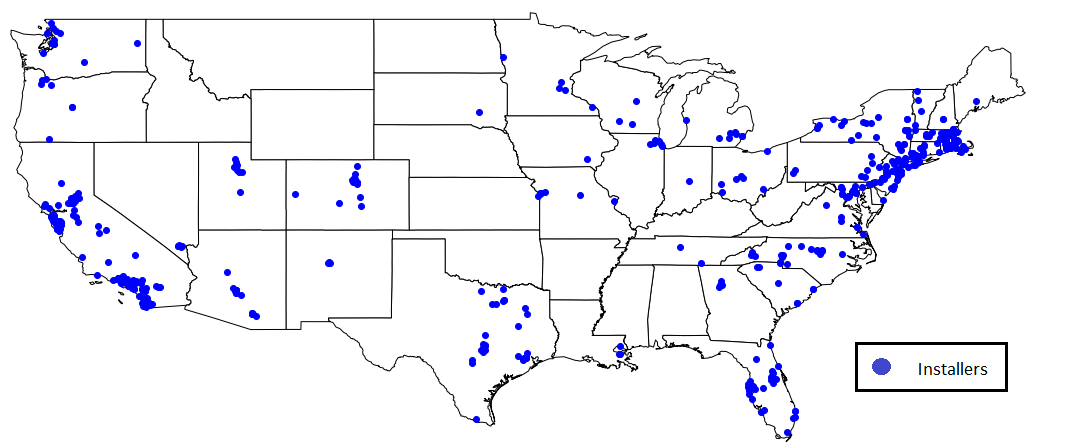
\includegraphics[width=1\linewidth]{national_installers.png}
	\caption{Installers in our data set}
	\label{fig: nationalinstallers}
\end{figure}


%We learned from our conversions with practitioners that the online marketplace actively reaches out to solar installers to encourage them to join the platform and help them set up their profiles. So, unlike starting a physical business, installers' fixed cost of entry to the online marketplace is negligibly small (if not zero). This is indeed the case in many other platforms \citep{haddad2015consumer}. Because there is almost no barrier for entry to the online marketplace, we study installers' activity levels after they establish their profiles on the marketplace; we do not explicitly model installers' entry decisions in the marketplace.


%Lastly, we don't observe quitting the platform the same way as physical store closes off. We simply observe inactive profiles. Thus we do not explicitly investigate the exit behavior.


\subsection{Defining Local Market}
\label{defining_local_market}


Solar installation is a combination of product and service. As part of service, installers typically visit customer site multiple times. Thus, each installer only operates  within a certain geographical area, and installers compete ``locally.'' That is, they only compete with installers that are relatively nearby. There is no data on the installers' service areas. To capture this practical element, we identify what is called \emph{local markets} within the marketplace so that only installers in the same local market compete with each other.

To geographically segment the marketplace into local markets, we divide installers into multiple \emph{clusters} and treat each cluster as a separate local market. Boundaries of local markets cannot be simply defined by city, county, or congressional district borders because it is common for installers to cross these artificial borders to serve customers. Instead, we use installer locations and the state-of-the-art advanced clustering algorithm called OPTICS (short for \textit{Ordering Points To Identify the Clustering Structure}) to identify local markets.

The OPTICS routine is an unsupervised machine learning algorithm that identifies density-based clusters in spatial data. It is considered to be an extension of various commonly-used advanced clustering algorithms, such as the DBSCAN \citep{kanagala2016comparative}. Among others, an important advantage of the OPTICS algorithm is that it does not require setting the number of clusters before running the algorithm as in $k$-means clustering; rather, it identifies the optimal number of clusters using the data. Because of its advantages, it has been applied in various contexts, ranging from political science \citep{davidson2019neighborhood} to geography \citep{teimouri2016method}.

%data mining \citep{breunig2000fast},

In light of these, we create the geographic division of local markets with the following steps. First, we collected the 5-digit zipcode of
every installer in the marketplace. Figure \ref{fig: nationalinstallers} displays the location of every installer in our data set. We then converted each zipcode  to the representative coordinates based on the data provided by the \citet{us_census_bureau_2019}. \textbf{IS THE FOLLOWING SENTENCE CORRECT? PLEASE CONFIRM:} This transformation is necessary to run the OPTICS algorithm on the location data. The OPTICS algorithm uses the maximum distance between two samples in a cluster as an input variable. Based on our conversations with practitioners, we learned that the majority of customers get a quote from an installer within 90 miles distance of their property. Consistent with this, we used 90 miles as the maximum distance input parameter, and the OPTICS algorithm generated 36 clusters. Each of these clusters geographically defines a local market boundary. Figure \ref{fig: markets} illustrates the centroid of each of these 36 clusters, which represents the centroid of each local market. Hereafter, for brevity, we refer to local markets simply as ``\emph{markets}.''

%\footnote{We also checked the robustness of our results by taking the maximum distance parameter as 100 miles in the OPTICS algorithm. Our insights remain to be valid with that alternative parameter.}



%\paragraph{OPTICS}  The OPTICS algorithm, short for \textit{Ordering Points To Identify the Clustering Structure}, is what we use to cluster installers' coordinates. The OPTICS routine is completed with the following parameter considerations:  \\
%\textbf{min samples: }
%The number of samples in a neighborhood for a point to be considered as a core point.  We use 2 as the default value.
%\textbf{metric}: haversine distance. Although not ideal, it better reflected the distance between two Latitude/Longitude points and is still fast enough in the clustering algorithm.  \textbf{max eps:} The maximum distance between two samples for one to be considered as in the neighborhood of the other. According to the survey that the marketplace conducted, 90.6 percent of customers get a quote from an installer within 100 miles of their property ( 81.7 percent from 50 miles). \citep{marsh_2019} We used 90 as the parameter to balance between having enough clusters to  make use of the inherent variations and make sure each cluster captured the local market condition. We use this cluster to define our market boundary geographically. Figure \ref{fig:markets} illustrates the centroid of each of these 36 clusters, which represents the centroid of each local market. Hereafter, for brevity, we refer to local markets simply as ``\emph{markets}.''



%(PROVIDE A PICTURE TO ILLUSTRATE THE CALINSKI-HARABASZ CURVE VS PARAMETER , refer to figure \ref{optics_parameter_gridsearch} and Calinski-Harabasz criteria : \citep{calinski1974dendrite}.





%\begin{figure}
%	\centering
%	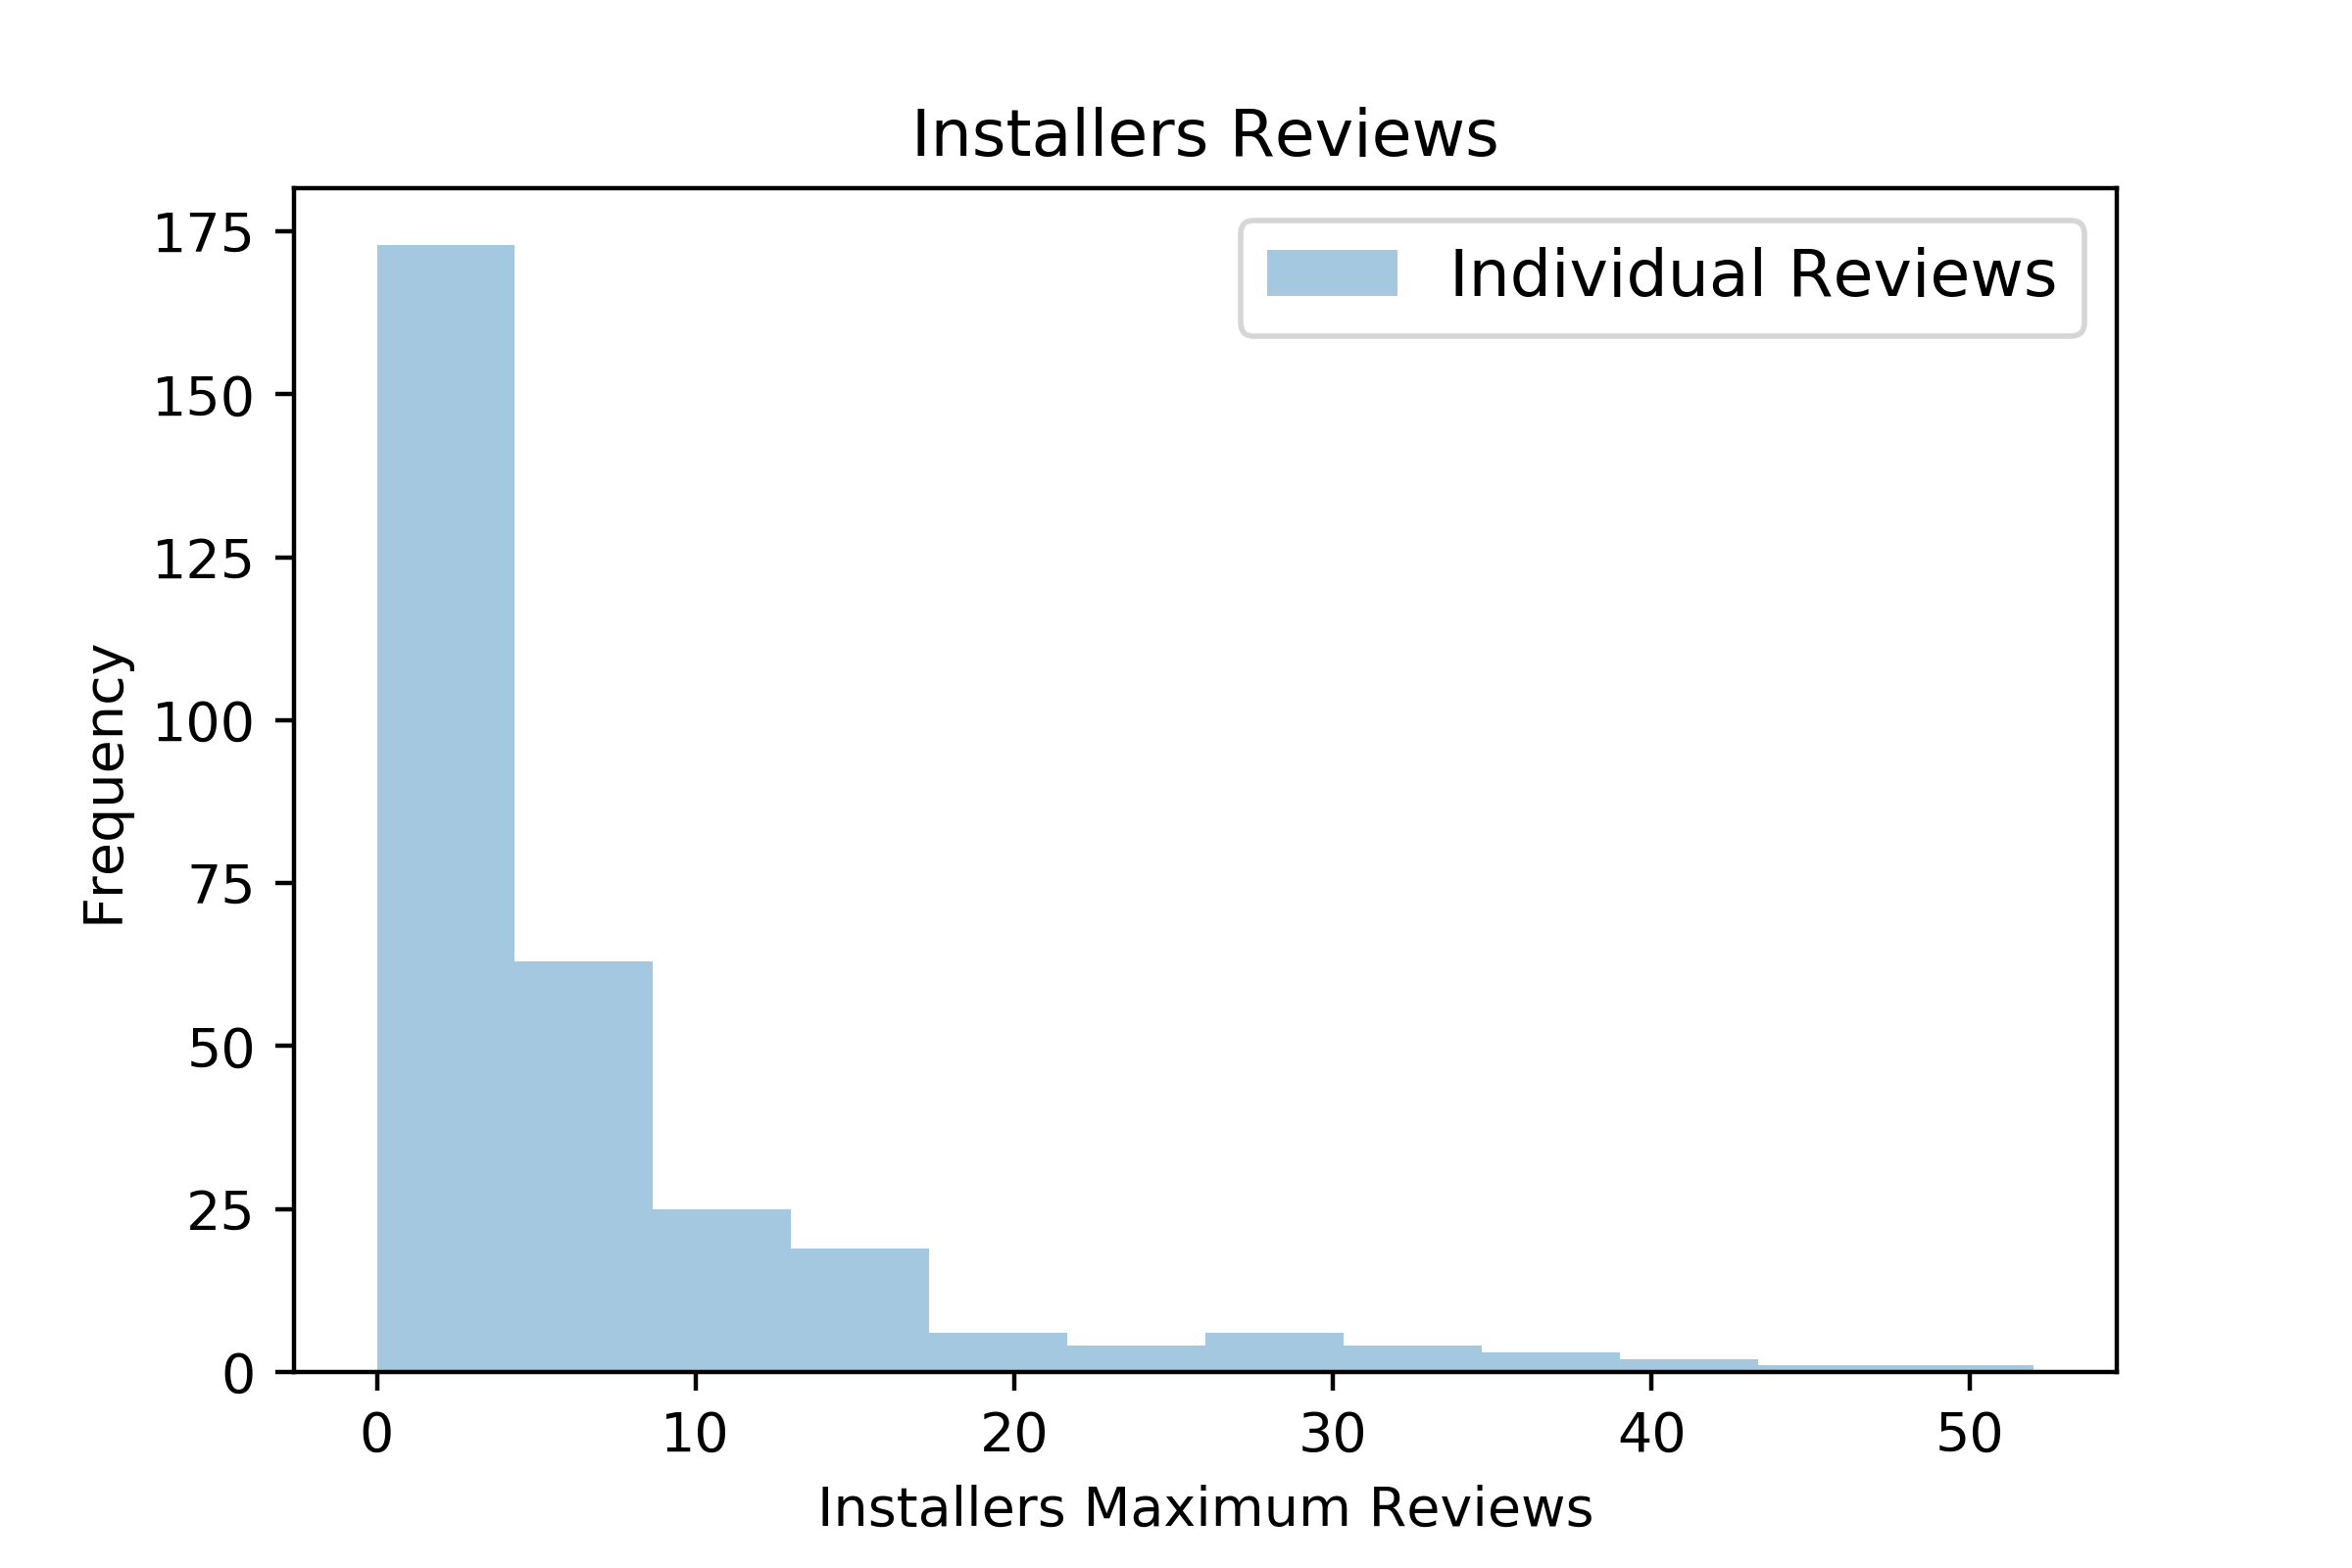
\includegraphics[width=1\linewidth]{histogram_ind_max_reviews_ct.png}
%	\caption{Reviews Histogram by Installer}
%	\label{histogram_ind_max_reviews_ct}
%\end{figure}
%
%% Please add the following required packages to your document preamble:
% \usepackage{booktabs}
\begin{table}
\centering
\begin{tabular}{@{}ccccc@{}}
\toprule
 & Unique  & Total Number & Total Number     & Total Number   \\
State    & Installers & of Reviews   & of Installations & of Quotes \\ \midrule  
CO & 13 & 799  & 168  & 13276 \\
MD & 10 & 895  & 144  & 4054  \\
WA & 9  & 902  & 35   & 1266  \\
TX & 27 & 987  & 90   & 12557 \\
FL & 21 & 994  & 141  & 9047  \\
CT & 10 & 1037 & 78   & 2746  \\
NC & 16 & 1100 & 95   & 7066  \\
NJ & 26 & 1674 & 223  & 8215  \\
NY & 32 & 2790 & 265  & 15128 \\
MA & 36 & 3519 & 507  & 19028 \\
CA & 95 & 7703 & 1472 & 98597 \\ \bottomrule
\end{tabular}
\caption{Top 10 States }
\label{summarystats_top10states}
\end{table}
%
%
%
\begin{figure}
	\centering
	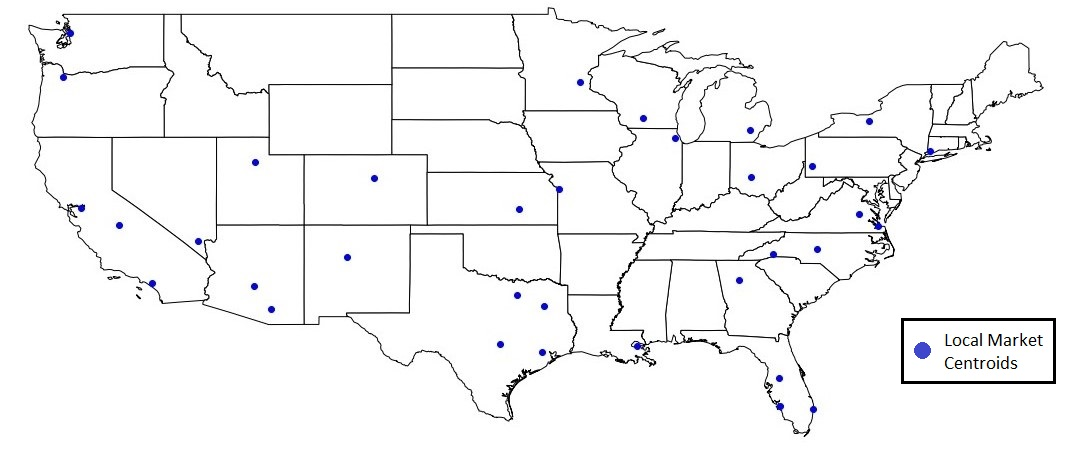
\includegraphics[width=1\linewidth]{markets.jpg}
	\caption{Local Market Centroids}
	\label{fig: markets}
\end{figure}

\subsection{Measuring Dispersion in Customer Ratings} \label{Subsec: Measure Dispersion}

A key explanatory variable in our base regression is the dispersion in customer ratings. This section explains how we measure the rating dispersion. Later, we will also study an extended model by adding the text-based review dispersion as a separate variable in our analysis.  Section \ref{Sec: TextMining} will explain the state-of-the-art natural language processing model we use to measure the review dispersion based on text data.

%\subsubsection{Measuring Rating-Based Dispersion} \label{Subsec: Define Ent}

We measure the rating dispersion by calculating the \emph{entropy} of ratings. In information theory, the entropy is a common way to measure  the uncertainty in a random variable's possible realizations. In our setting, because the marketplace has a 5-star rating system, the entropy of ratings is
\begin{equation}\label{def: entropy}
H(R)=-\sum_{i=1}^{5} \text{Prob}(\text{Rating}=i) \ln(1/\text{Prob}(\text{Rating}=i)).
\end{equation}
For example, for a set of 5 reviews each with 4 stars (out of 5 stars), the entropy of ratings $\{4,4,4,4,4\}$ is zero. Alternatively, for a set of 5 reviews with ratings $\{3,5,3,5,4\}$, the entropy of ratings is 1.0549. Although both sets have the same average rating of 4, the latter set of ratings provides more information with a higher dispersion, hence has a higher entropy.


In light of this, we create three variables that measure the rating entropy in different dimensions for each month $t$. First variable is $\text{Rating\_Entropy\_Self}_{i,t}$, which is the demeaned entropy of each installer $i$'s own ratings. This is calculated on the set of reviews that are associated with installer $i$ up to \textbf{PLEASE CONFIRM: and including} month $t$. Recalling the market defined in Section \ref{defining_local_market}, the second variable is $\text{Rating\_Entropy\_Others}_{i,t}$ that is the demeaned rating entropy of all other installers in installer $i$'s market, up to and \textbf{and including} month $t$. In one of our sections, we will consider the demeaned rating entropy on the market level. Thus, our third variable is $\text{Rating\_Entropy\_Mkt}_{m,t}$ that represents the demeaned entropy of all ratings in the local market $m$, up to  \textbf{and including} month $t$. Note that these three variables are centered around their means. This is a standard procedure in setting like ours where the regression allows for both linear and quadratic versions of the same independent variable (see, e.g., \citep{tan2014does}). We also checked the robustness of our findings by replacing these variables with their non-demeaned versions in all our econometric analysis, and we find that all of our insights remain the same with non-demeaned variables.

We measure the rating dispersion by calculating entropy rather than variance or coefficient of variation of ratings. The reason is two folds: First, the variance and coefficient of variance of ratings are both very highly correlated with average ratings. (The aforementioned correlation is more than 0.7.) In contrast, rating entropy exhibits a much lower level of correlation with average ratings. Thus, measuring the rating dispersion via the rating entropy enables us to include both rating dispersion and average rating as explanatory variables in our model. \textbf{PLEASE CLARIFY: Second, entropy measure is more appropriate for capturing data that are potentially multimodal \citep{smaldino2013measures}.}  


%********** COPY PASTE ICIN******
%
%We transformed $\text{Installer\_Activity}$ and $\text{Market\_Transaction}$ into their natural logarithm. Natural log transformation on continuous dependent variable is a commonly used technique that is embraced by similar work such as \citep{tan2019you}. The distribution of the $\text{Installer\_Activity}$ and $\text{Market\_Transaction}$ are right-skewed with a skewness of $6.9$ and $6.1$ respectively. We transform the data to better conform to normality in order to improve the validity of inference.  As a robustness check, we performed analysis without log transformation and the results are consistent.




\section{Installer-Level Analysis \& Results} \label{Sec: Installer-level}

This section examines the following questions: (i) How does the dispersion in an installer's ratings affect its \emph{activity level}, which is the logged  number of proposals generated by the installer? (ii) How does the dispersion in competitors' ratings impact the installer's activity level? By studying these questions, we test Hypotheses 1a, 1b, 2a and 2b in Section \ref{Sec: Hypothesis}.


We will only use numerical ratings in this section. Later, in Section \ref{Sec: TextMining}, we will also use text reviews in our analysis. We will check the robustness of our findings in various dimensions, and address potential endogeneity concerns in an extended model in Section \ref{Sec: Robustness}.

\subsection{Regression Equation \& Controls}

 To answer (i) and (ii) above, we run a regression model where the dependent variable is the natural logarithm of the number of proposals made by the installer. Specifically, indexing installers, months and markets by $i$, $t$ and $m$, respectively, the dependent variable in our regression is  $\text{Installer\_Activity}_{i,m,t+1}$, which is equal to $\log$(1 $+$ number of proposals generated by installer $i$) in the market $m$ during month $t$+1. We take the natural logarithm transformation of the number of proposals because its distribution is right-skewed.  We transform the data to increase the normality of errors, thereby further improve the validity of inference. This transformation is a standard technique in the literature (see, e.g., \citet{song2017closing,tan2014does}, among others). As a robustness check, we performed the analysis without log transformation and the results are consistent.

 Two of our key independent variables are $\text{Rating\_Entropy\_Self}_{i,t}$ and  $\text{Rating\_Entropy\_Others}_{i,t}$, which are the rating entropy variables defined in Section \ref{Subsec: Measure Dispersion}. Because we have competing hypotheses, we also allow for nonlinear relationships between these independent variables and the dependent variable. Thus, we include explanatory variables $\text{Rating\_Entropy\_Self}_{i,t}^{2}$ and $\text{Rating\_Entropy\_Others}_{i,t}^{2}$ in our regression, as well:
\begin{align}  \nonumber
    \text{Installer\_Activity}_{i,m,t+1}=&\beta_{0}+\beta_{1} \text{Rating\_Entropy\_Self}_{i,t}+\beta_{2} \text{Rating\_Entropy\_Self}_{i,t}^ {2}
    \\ \nonumber
    &+\beta_{3} \text{Rating\_Entropy\_Others}_{i,t}  +\beta_{4}\text{Rating\_Entropy\_Others}_{i,t}^{2} \\ \label{model_ind_3}
    &+ \text{Controls}_{i,m,t}+ \alpha_{i} + \epsilon_{i,t+1}.
\end{align}
 Here, $\epsilon$ is the installer-level error term, and represents random factors that are unobservable in the data and affect the installer activity.  We run two versions of \eqref{model_ind_3}: In one version, we consider $\alpha_{i}$ as a fixed effect whereas in the alternative version, we consider it as a random effect. To determine which model is more appropriate for our data, we run the Durbin-Wu-Hausman test where the null hypothesis is that the the random-effect model is preferred while the alternative is the fixed-effect model. With a p-value $<0.0001$, we reject the null hypothesis and conclude that the fixed-effect model is more appropriate. We also establish the significance of the fixed effect in \eqref{model_ind_3} with the $F$-test ( $\chi^{2}(13)=44.23,p<0.0001$) \textbf{PLEASE ENTER THE SIGNIFICANCE VALUE}). Thus, we focus on \eqref{model_ind_3} with the installer-level fixed effect $\alpha_{i}$ that controls for time-invariant characteristics of each installer.

In this regression model, the key coefficients of interests are $\beta_{1}$, $\beta_{2}$, $\beta_{3}$ and $\beta_{4}$. The values of these coefficients together with the significance of the associated variables will uncover how the rating entropy impacts the installer's activity level in the online platform.


 The regression \eqref{model_ind_3} includes various installer-level or market-level control variables ($\text{Controls}_{i,m,t}$).  To account for the state-level renewable policy effects, we include state dummies as control variables. We have 33 such variables. We account for the impact of the solar panel prices on installers' activity levels by considering $\text{Price\_Difference}_{i,t}$ as another control variable.  In practice, because solar PV systems vary in size, price per KW is a common way to represent the price of the installed solar panel. We use the TTS dataset to find each installer's price for 1 KW solar panel by matching names and zipcodes. Based on this, we compute the variable $\text{Price\_Difference}_{i,t}$ by taking the logarithm of the difference between installer $i$'s price and the average price of its competitors that operate in the same market in month $t$.  We control for the average rating of each installer $i$ as well as the average rating of its competitors in the market for month $t$ by including variables $\text{Average\_Rating\_Self}_{i,t}$ and $\text{Average\_Rating\_Others}_{i,t}$ in \eqref{model_ind_3}. We also control for the installer's experience by the control variable $\text{Experience}_{i,t}$ that is the logarithm of the number of years the installer has been installing solar systems up to (and including) month $t$. We collected this information from each installer's website. Another control variable in \eqref{model_ind_3} is $\text{Market\_LogRevenue}_{m,t}$  that measures the logged total dollar value of all solar installations within market $m$ during month $t$. To create this variable, we augment the market boundaries identified in Section \ref{defining_local_market} with the TTS data. This variable aims to capture total solar installations opportunities in the market, and can be seen as a proxy for the favorableness of the solar installation market. As the final control variable, we consider  $\text{Review\_Counts}_{i,t}$ which is the number of each installer $i$'s reviews up to (and including) month $t$.





% the following regression equation is used to estimate the impact of ratings dispersion (own ratings dispersion: $Ent_{i,self,t}$ ; others ratings dispersion: $Ent_{i,others,t}$) on focal installer's activity intensities $ActInt_{i,m,t}$:
%\begin{equation}
%    ActInt_{i,m,t+1}=\beta_{0}+\beta_{11} Ent_{i,m,others,t}+\beta_{2}Ent_{i,m,others,t}^2+
%   Controls_{i,t}+\alpha_{i}+\epsilon_{i,m,t}
%   \label{model_ind_1}
%\end{equation}
%
%\begin{equation}
%    ActInt_{i,m,t+1}=\beta_{3}+\beta_{4} Ent_{i,self,t}+\beta_{5}Ent_{i,self,t}^2+
%   Controls_{it}+\alpha_{i}+\epsilon_{i,m,t}
%   \label{model_ind_2}
%\end{equation}

Tables \ref{sumstats_ind} and \ref{corr_ind} below present the summary statistics and the correlation matrix. By Table \ref{corr_ind}, correlations among explanatory variables are relatively low and do not hurt the validity of regression analysis.

% Please add the following required packages to your document preamble:
% \usepackage{booktabs}
% \usepackage{graphicx}
\begin{table}[H]
\centering
\begin{tabular}{@{}lccccc@{}}
\toprule
Variables               & N     & Mean    & Standard Deviation & Min    & Max   \\ \midrule
Rating\_Entropy\_Self   & 4,562 & 0  & 0.217  & -0.0985 & 0.9015     \\
Rating\_Entropy\_Others & 4,562 & 0   & 0.183  & -0.227  & 0.773     \\
Average\_Rating\_Self   & 4,562 & 4.531   & 1.316  & 1      & 5     \\
Average\_Rating\_Others & 4,562 & 4.88    & 0.205  & 1      & 5     \\
Review\_Count           & 4,562 & 5.384   & 6.836  & 0      & 52    \\
Experience              & 4,562 & 1.758   & 0.929  & 0      & 3.714 \\
Price\_Difference       & 4,562 & -0.0333 & 0.392  & -2.171 & 3.139 \\
Market\_LogRevenue      & 4,562 & 12.24   & 7.9    & 0      & 22.3  \\ \bottomrule
\end{tabular}%
\caption{Summary Statistics - Installer Level Analysis}
\label{sumstats_ind}
{\footnotesize \textit{Note: All entropy variables are demeaned.}}
\end{table} 

% Please add the following required packages to your document preamble:
% \usepackage{booktabs}
% \usepackage{graphicx}
\begin{table}[H]
\centering
\begin{tabular}{@{}lllllllll@{}}
\toprule
Variables                   & (1)    & (2)    & (3)    & (4)    & (5)    & (6)    & (7)        & (8)     \\ \midrule
(1) Rating\_Entropy\_Self   & 1      & \multicolumn{7}{l}{}                                              \\
(2) Rating\_Entropy\_Others & -0.094 & 1      & \multicolumn{6}{l}{}                                     \\
(3) Average\_Rating\_Self   & -0.088 & 0.069  & 1      & \multicolumn{5}{l}{}                            \\
(4) Average\_Rating\_Others & 0.025  & -0.523 & -0.017 & 1      & \multicolumn{4}{l}{}                   \\
(5) Review\_Count           & 0.241  & 0.061  & 0.205  & -0.039 & 1      & \multicolumn{3}{l}{}          \\
(6) Experience              & -0.001 & 0.143  & 0.036  & -0.062 & 0.127  & 1      & \multicolumn{2}{l}{} \\
(7) Price\_Difference       & -0.015 & -0.043 & 0.003  & 0.016  & -0.029 & -0.027 & 1          &         \\
(8) Market\_LogRevenue      & -0.026 & 0.006  & -0.029 & 0.044  & -0.086 & 0.451  & -0.059     & 1       \\ \bottomrule
\end{tabular}%
\caption{Correlation Matrix - Installer Level Analysis}
\label{corr_ind}
\end{table} 

\subsection{Results}

Table \ref{reg_ind_all} presents the results estimated by three panel regression models based on the equation \eqref{model_ind_3}. Columns (I) through (III) of Table \ref{reg_ind_all} present the estimates obtained by using different set of explanatory variables in the regression. The column (III) includes the estimates under the regression model \eqref{model_ind_3}, while the estimates in other columns are obtained by considering only some of these variables in the regression. In particular, we obtain the estimates in column (I) in the absence of all entropy variables in \eqref{model_ind_3}; column (II) presents the estimates when we exclude variables related to the installer's rating entropy from \eqref{model_ind_3}.


% Please add the following required packages to your document preamble:
% \usepackage{booktabs}
% \usepackage{graphicx}
\begin{table}[]
\centering
\begin{threeparttable}
\begin{tabular}{@{}lccc@{}}
\toprule
                  & (I)      & (II)    & (III)   \\  
& Installer's Activity & Installer's Activity & Installer's Activity \\
Variables & Level    & Level   & Level   \\ \midrule
Rating\_Entropy\_Self                                &                            &                            & 1.890***                   \\
                                                     &                            &                            & (0.000)                    \\
Rating\_Entropy\_Self$^2$                            &                            &                            & -3.473***                  \\
                                                     &                            &                            & (0.000)                    \\
Rating\_Entropy\_Others                              &                            & 0.524**                    & 0.488**                    \\
                                                     &                            & (0.004)                    & (0.007)                    \\
Rating\_Entropy\_Others$^2$                          &                            & -2.533***                  & -2.593***                  \\
                                                     &                            & (0.000)                    & (0.000)                    \\
Average\_Rating\_Self                                & -0.876***                  & -0.834***                  & -0.774**                   \\
                                                     & (0.000)                    & (0.000)                    & (0.001)                    \\
Average\_Rating\_Others                              & 0.000618                   & 0.000236                   & 0.000964                   \\
                                                     & (0.975)                    & (0.991)                    & (0.963)                    \\
Review\_Count                                        & 0.0561***                  & 0.0534***                  & 0.0472***                  \\
                                                     & (0.000)                    & (0.000)                    & (0.000)                    \\
Experience                                           & 0.218***                   & 0.212***                   & 0.206***                   \\
                                                     & (0.000)                    & (0.000)                    & (0.000)                    \\
Price\_Difference                                    & 0.0593                     & 0.0690                     & 0.0722                     \\
                                                     & (0.487)                    & (0.425)                    & (0.402)                    \\
Market\_LogRevenue                                   & -0.0168***                 & -0.0169***                 & -0.0159***                 \\
                                                     & (0.000)                    & (0.000)                    & (0.001)                    \\
Constant                                             & 2.690***                   & 2.803***                   & 2.961***                   \\
                                                     & (0.000)                    & (0.000)                    & (0.000)                    \\
Observations                                         & 4562                       & 4562                       & 4562                       \\
Fixed Effect                             & Yes        & Yes        & Yes       \\
State Dummies                            & Yes        & Yes        & Yes       \\
Adjusted R$^2$                                                     & 0.627                      & 0.630                      & 0.633       \\
AIC                                                  & 13267.2                    & 13234.9                    & 13205.7                    \\
BIC                                                  & 13325.0                    & 13305.6                    & 13289.2                    \\ \bottomrule

\end{tabular}%
\begin{tablenotes}
\item Note: $p$-value in parentheses; $^\star p<0.05;^{\star\star} p<0.01;^{\star\star\star} p<0.001 $
\end{tablenotes}
\caption{Installer Level Analysis}
\label{reg_ind_all}
\end{threeparttable}
\end{table}

Our estimates in Table \ref{reg_ind_all} identify three key results. First, the set of variables representing ``noise'' or dispersion of ratings have a significant impact on an installer's activity level in the marketplace. This is because in the column (III) of Table \ref{reg_ind_all}, all entropy variables are found to be statistically significant.

Second, the dispersion in an installer's ratings has a positive and statistically significant first-order effect on the installer's activity level because in the column (III), the variable ``Rating\_Entropy\_ Self'' is found to be significant and its coefficient is positive ($\beta_{1} = 1.890,p<0.001$). However, we also find that an installer's rating dispersion has a negative and statistically significant second-order effect on its activity level. The reason is that in the column (III), the variable ``Rating Entropy Self$^2$'' is significant and its coefficient is negative ($\beta_{2} = -3.473, p<0.001$). Combining these two effects, the regression estimates indicate that the dispersion in an installer's ratings has a concave and non-monotone impact on the installer's activity level in the online marketplace. Specifically,  an installer's rating dispersion increases its activity level in the online marketplace if and only if the aforementioned dispersion is below a threshold. When the dispersion of its ratings exceeds that threshold, any additional dispersion in the installer's ratings deters its activity in the marketplace. These provide support for Hypothesis 1A if and only if the installer's rating entropy is smaller than a threshold; otherwise, our findings are in support of Hypothesis 1B.

Third,  our estimation shows that the entropy of competitors' ratings impacts an installer's activity level in the same way as the entropy of the installer's ratings. Specifically, it has a positive and significant first-order effect (as ``Rating\_Entropy\_Others'' is significant and its coefficient $\beta_{3} =  0.488$ ($p<0.01$), and a negative and significant second-order effect (as ``Rating\_Entropy\_Others$^{2}$'' is significant and its coefficient $\beta_{4} = -2.593, p<0.001$). Combining these two effects,
 the dispersion in competitors' ratings increases the installer's activity level if and only if the aforementioned dispersion is below a threshold. When the dispersion of competitors' ratings is above that threshold, any additional dispersion in competitors' ratings deters the installer's activity in the marketplace. This implies support for Hypothesis 2A if and only if the competitors' rating entropy is below the threshold; otherwise, our findings offer support for Hypothesis 2B.


Figures \ref{fig: marginsplot_ind_ent_self} and  \ref{fig: marginsplot_ind_ent_others} illustrate the explained nonlinear effects of the rating entropy on the installer's activity level in the online marketplace. In generating Figures \ref{fig: marginsplot_ind_ent_self} and  \ref{fig: marginsplot_ind_ent_others}, we use the estimated regression coefficients in the column (III) of Table \ref{reg_ind_all}. As is apparent from these figures, on average, the installer's activity level first increases and then decreases with its rating entropy (or the rating entropy of its competitors), yielding an inverted U-shaped relationship between the two.

\begin{figure}
	\centering
	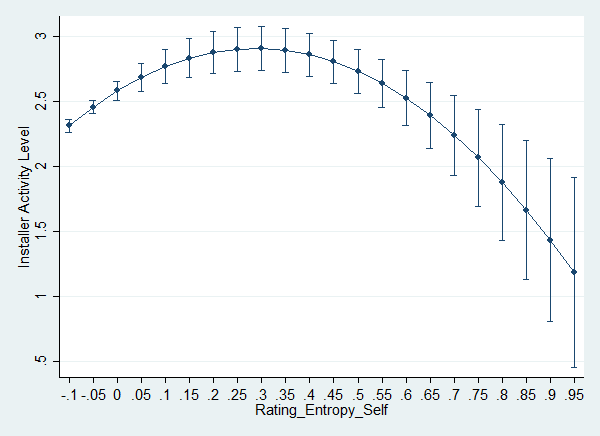
\includegraphics[width=0.7\linewidth]{marginsplot_entself.png}
	\caption{Predictive value of the Entropy of the Installer's Own Ratings on its Activity Level}
	\label{fig: marginsplot_ind_ent_self}
\end{figure}

\begin{figure}
	\centering
	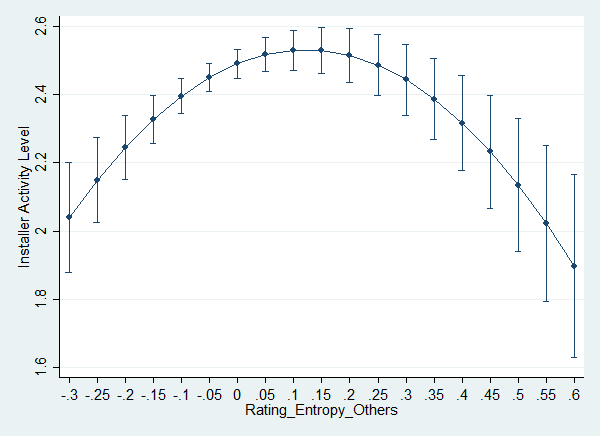
\includegraphics[width=0.7\linewidth]{marginsplot_entothers.png}
	\caption{Predictive value of Other Installers' Rating Entropy (in the same market) on the Installer's Activity Level}
	\label{fig: marginsplot_ind_ent_others}
\end{figure}





Finally, in all three columns of Table \ref{reg_ind_all}, the installer's average rating is significantly and negatively linked with its activity level. Put another way, installers appear to extend fewer proposals as their average ratings increase. One reason for this behavior could be that  installers become more selective after they attain a high average rating in the marketplace. Selectiveness can emerge because the installers might think that with a higher average rating, their proposals are more likely to be accepted by customers, and thus making too many offers increases their likelihood of coming across with a negative customer.

\section{Market-Level Analysis \& Results} \label{Sec: Market-level}

An important performance metric for the marketplace operator is the number of matches (i.e., agreed proposals) between installers and customers in the marketplace. This section estimates how the market-level rating dispersion impacts the \emph{market transaction} that is the logged number of matches in the market. With this, we test Hypotheses 3A and 3B in Section \ref{Sec: Hypothesis}.

We will only use numerical ratings in this section. As an extension, Section \ref{Sec: TextMining} will account for text reviews in the market-level analysis. We will provide various additional robustness checks of our findings, and address potential endogeneity concerns in an extended model in Section \ref{Sec: Robustness}.



Recalling that markets and months are indexed by $m$ and $t$, respectively, we use the following regression equation for the estimation:
\begin{align} \nonumber
   \text{Market\_Transaction}_{m,t+1} & =\beta_{5} + \beta_{6} \text{Rating\_Entropy\_Mkt}_{m,t}+ \beta_{7} \text{Rating\_Entropy\_Mkt}_{m,t}^2\\ \label{reg: market-level-rating}
   &+ \text{Controls}_{m,t}  +\epsilon_{m,t+1}.
\end{align}

Performing \eqref{reg: market-level-rating} requires us to convert the installer-level monthly panel data to the market-level monthly panel data based on the markets defined in Section \ref{defining_local_market}. Our data include the number of agreed proposals for each installer $i$ in each month $t$. To create our dependent variable $\text{Market\_Transaction}_{m,t+1}$, we first calculate the total number of proposals accepted by customers in market $m$ and month $t+1$, and then take the logarithmic transformation of that sum. Formally, $\text{Market\_Transaction}_{m,t+1} =$ $\log\left( \sum_{i \in \text{Market\ } m} \text{Successful\_Proposals}_{i}+ 1 \right)$ in \eqref{reg: market-level-rating}.  We employ this standard transformation because the number of matches is right-skewed and the transformation increases the normality of errors. (As a robustness check, we also perform the analysis without log transformation and the results are consistent.)

A key explanatory variable in \eqref{reg: market-level-rating} is $\text{Rating\_Entropy\_Mkt}_{m,t}$, which is the entropy of all installers' ratings up to (and including) month $t$ in the market $m$.
 Because we have two competing hypotheses about the impact of market-level rating entropy (i.e., Hypotheses 3A and 3B in Section \ref{Sec: Hypothesis}), we also allow for a  nonlinear relationship between the market-level rating entropy and the dependent variable. Thus, \eqref{reg: market-level-rating} also contains the quadratic term  $\text{Rating\_Entropy\_Market}_{m,t}^{2}$. The aforementioned two variables are our main explanatory variables, and $\beta_{6}$ and $\beta_{7}$ are the key coefficients of interests. The values of these coefficients together with the significance of the associated explanatory variables will help us determine how the market-level rating entropy impacts market transactions.


 In \eqref{reg: market-level-rating}, $\epsilon$ is the market-level error term, and represents random factors that are unobservable in the data and affect market transactions. We also use various control variables ($\text{Controls}_{m,t}$) in \eqref{reg: market-level-rating}. We control for the state of the market. To do that, we created 33 state dummies to represent 33 different states included in the data set. In our dataset, 18\% of markets span across more than one state.  In light of this, each state dummy represents the fraction of installers that are located in that state within the market $m$. For example, suppose market 1 has 25\% of installers from state X and 75\% from Y. Then, we assign 0.25 to the dummy variable State\_X and 0.75 to the dummy variable State\_Y for market 1.  Similar to the installer-level analysis in Section \ref{Sec: Installer-level}, we created the variable $\text{Average\_Experience}_{m,t}$ that represents the average experience of installers in the market $m$ up to and including month $t$. We calculated this by averaging installers' experience levels across the market $m$. In parallel to the installer-level analysis, we use the variable $\text{Average\_Rating\_Mkt}_{m,t}$ to control for the average rating of all installers in the market $m$ until (and including) month $t$. As another control, we created the variable $\text{Review\_Count\_Mkt}_{m,t}$ that measures the total number of reviews by all installers in the market $m$ up to and including month $t$. We also control for the difference between the average unit price of installed 1 KW solar system in the marketplace and off-marketplace, which is represented by the variable $\text{Price\_Difference\_Mkt}_{m,t}$. Finally, we use $\text{Market\_LogRevenue}_{m,t}$ as a control where it is as defined in Section \ref{Sec: Installer-level}. Summary statistics can be found in Table \ref{sumstats_mkt}; the correlation coefficients among variables are presented in Table \ref{corr_mkt}.



\subsection{Results}


Table \ref{reg_mkt_simplified} presents our regression estimates. In Table \ref{reg_mkt_simplified}, column (I) shows the estimates obtained with the regression \eqref{reg: market-level-rating} in the absence of $\text{Rating\_Entropy\_Mkt}_{m,t}$ and $\text{Rating\_Entropy\_Mkt}^2_{m,t}$ variables, while column (II) includes the estimates obtained by running the regression \eqref{reg: market-level-rating} considering all variables in \eqref{reg: market-level-rating}.
% Please add the following required packages to your document preamble:
% \usepackage{booktabs}
% \usepackage{graphicx}
\begin{table}[H]
\centering

\begin{tabular}{@{}lccccc@{}}
\toprule
Variables            & N   & Mean   & Standard Deviation & Min    & Max   \\ \midrule
Rating\_Entropy\_Mkt & 642 & 0  & 0.236              & -0.191  & 0.809    \\
Market\_LogRevenue   & 642 & 7.887  & 8.102               & 0      & 22.3  \\
Average\_Rating\_Mkt & 642 & 4.870  & 0.245              & 3      & 5     \\
Average\_Experience  & 642 & 1.426 & 1.110              & 0      & 3.332    \\
Price\_Difference\_Mkt    & 642 & -0.0106 & 0.146              & -0.504 & 1.312 \\ \bottomrule
\end{tabular}%

\caption{Summary Statistics - Market Level Analysis}
\label{sumstats_mkt}
\end{table} 
% Please add the following required packages to your document preamble:
% \usepackage{booktabs}
% \usepackage{graphicx}
\begin{table}[H]
\centering
\begin{tabular}{@{}llllll@{}}
\toprule
Variables                & (1)    & (2)    & (3)    & (4)    & (5) \\ \midrule
(1) Rating\_Entropy\_Mkt & 1      &        &        &        &     \\
(2) Average\_Rating\_Mkt & -0.624 & 1      &        &        &     \\
(3) Average\_Experience  & 0.198  & -0.107 & 1      &        &     \\
(4) Price\_Difference\_Mkt    & -0.018 & -0.041 & -0.012 & 1      &     \\
(5) Market\_LogRevenue   & 0.157  & -0.041 & 0.498  & -0.126 & 1   \\ \bottomrule
\end{tabular}
\caption{Correlation Matrix - Market Level Analysis}
\label{corr_mkt}
\end{table} 
% Please add the following required packages to your document preamble:
% \usepackage{booktabs}
% \usepackage{graphicx}
\begin{table}[]
\centering
\begin{threeparttable}[t]
\begin{tabular}{@{}lcc@{}}
\toprule
                                    & (I)                   & (II)                  \\
Variables                                    & Market Transaction & Market Transaction\\ \midrule
Rating\_Entropy\_Mkt                         &                       & 1.060***              \\
                                             &                       & (0.000)               \\
Rating\_Entropy\_Mkt$^2$                     &                       & -1.610***             \\
                                             &                       & (0.000)               \\
Average\_Rating\_Mkt                         & -0.273                & -0.185                \\
                                             & (0.071)               & (0.212)               \\
Average\_Experience                          & 0.0197*               & 0.0138                \\
                                             & (0.013)               & (0.073)               \\
Price\_Difference\_Mkt                       & 0.239                 & 0.287                 \\
                                             & (0.282)               & (0.194)               \\
Market\_LogRevenue                           & -0.0846               & -0.0663               \\
                                             & (0.057)               & (0.123)               \\
Constant                                     & 3.443**               & 2.909*                \\
                                             & (0.009)               & (0.025)               \\
Market Fixed Effect                          & Yes                   & Yes                   \\
Weighted State Dummies                       & Yes                   & Yes                   \\
Observations                                 & 642                   & 642                   \\
Adjusted R$^2$                                  & 0.739                 & 0.747                 \\
AIC                                          & 1075.6                & 1059.6                \\
BIC                                          & 1156.0                & 1148.9                \\ \bottomrule
\end{tabular}%
\begin{tablenotes}
\item Note: $p$-value in parentheses; $^\star p<0.05;^{\star\star} p<0.01;^{\star\star\star} p<0.001 $
\end{tablenotes}
\caption{Market Level Analysis}
\end{threeparttable}
\label{reg_mkt_simplified}
\end{table} 



Regression estimates reveal the following key findings. First, the dispersion (``noise'') in the market-level ratings has a significant and positive first-order effect on market transactions and number of matches in the market. This is because the coefficient of ``$\text{Rating\_Entropy\_Mkt}$'' is positive ($\beta_{6}=1.060$) and statistically significant ($p<0.01$) in the column (II) of Table \ref{reg_mkt_simplified}. The market-level rating dispersion also has a significant and negative second-order effect as the coefficient of the quadratic term ``$\text{Rating\_Entropy\_Mkt}^2$'' is negative ($\beta_{7}=-1.160$) and statistically significant ($p<0.01$) in the column (II). Combining these two effects, on average, regression estimates indicate a concave and non-monotone relationship between the market-level rating dispersion and the market transaction.  Specifically, our findings indicate that the market-level dispersion increases the market transaction and number of matches if and only if the mentioned dispersion is smaller than the threshold, for any dispersion beyond that threshold, any additional dispersion on the market-level dampens the market transaction and matches. These findings support Hypothesis 3A if and only if the market-level rating dispersion is below a certain threshold; our results are in support for Hypothesis 3B for any market-level dispersion above that threshold.

Figure \ref{fig: marginsplot_mkt_entmkt} further illustrates this nonlinear relationship via a margins plot using coefficients generated from estimates in the column (II) of Table \ref{reg_mkt_simplified}. As we observe from this figure, on average, the market transaction (and the number of matches) first increases then decreases with the market-level rating dispersion.

Finally, market-level estimates in Table \ref{reg_mkt_simplified} suggest that after controlling for market conditions, installer experience, price, and state, the average rating is not significantly associated with the market-level performance.
\begin{figure}
	\centering
	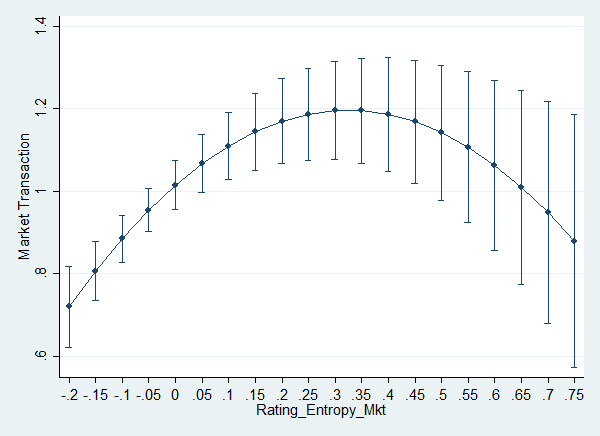
\includegraphics[width=0.7\linewidth]{marginsplot_entmkt.png}
	\caption{Marginal Impact of Market Reviews Entropy of Reviews on Market Level Matching}
	\label{fig: marginsplot_mkt_entmkt}
\end{figure}


\section{Text Mining}\label{Sec: TextMining}

In this section, we incorporate various methods to leverage rich text information in reviews.  First, we will use the state-of-the-art advanced natural language processing (NLP) technique called BERT (i.e., \textit{Bidirectional Encoder Representations from Transformers}) to measure the dispersion in text reviews. The BERT method was developed by Google AI in 2018, and incorporated by  Google Search Engine in late 2019 \citep{devlin2018bert,BERT}. To the best of our knowledge, there is no other paper in operations management literature that considers this technique. Second, we will use another state-of-the-art NLP method to generate the sentiment score of each review. As the final step, we will incorporate these text-based metrics in our regression analysis to derive additional insights related to the text content.

\subsection{Measuring Text-Based Review Dispersion via Natural Language Processing Technique BERT} \label{Subsec: Define Txt Ent}

In our data set, we have $3607$ pieces of text reviews, and we apply the following five steps to measure the dispersion in text reviews. First, we use BERT to convert each text review to a semantics-sensitive numerical vector. We will provide more details about this method later in this section.  As a second step, we normalize each vector to unit length. Third, we measure the cosine similarity between any two review vectors to find the context similarity between the two. The cosine similarity between two normalized vectors $V_{1}$ and $V_{2}$ equals the inner product of two, i.e., $V_1 \cdot V_2$, and gives the cosine of the angle between the two vectors. The angle represents the similarity in the orientation of two review vectors. For example, if the angle is $0$, the vectors are at the same orientation and hence the similarity is the maximum. The second and third steps above are standard in identifying the similarity between two vectors (see, e.g., \cite{hoberg2016text}). As the fourth step, we identify the cosine distance between every two review vectors using the fact that the cosine distance between the two normalized vectors $V_{1}$ and $V_{2}$ equals $1$ minus the cosine similarity between the two. This distance reflects how much two reviews differ from each other. As the fifth and final step, we calculate the dispersion of text reviews, i.e., \emph{text-based dispersion}, for a review set of interest by enumerating all pairwise cosine distances of reviews in that set and taking their statistical median (the 50$^{\text{th}}$ percentile). For example, for a set of 10 text reviews, we have 45 (=$\binom{10}{2}$) pairwise cosine distances. Finding the text-based dispersion for this set requires computing the median of these 45 distances. If these 10 pieces of texts are dissimilar from each other, they contain richer information and the median of these $45$ distances shall be higher; and vice versa.

 As a result of this procedure, similar to the rating entropy, we create the following three variables, each measuring the text-based dispersion in a different dimension: (i) $\text{Text\_Dispersion\_Self}_{i,t}$: Demeaned dispersion in installer $i$'s own text reviews up to and including month $t$. %Given $N_{i,t}$ pieces of text reviews available up to month $t$, it is calculated by computing $N_{i,t}\times (N_{i,t}-1)/2$ cosine distance pairs and taking the 50$^{th}$ percentile.
(ii) $\text{Text\_Dispersion\_Others}_{i,t}$: Demeaned dispersion in text reviews of all other installers in the installer $i$'s market up to and including month $t$. %Given $N_{-i,t}$ pieces of text reviews of other installers up to month $t$, it is calculated by computing $N_{-i,t}\times (N_{-i,t}-1)/2$ cosine distance pairs and taking the 50$^{th}$ percentile.
(iii) $\text{Text\_Dispersion\_Mkt}_{m,t}$: Demeaned dispersion in text reviews of all installers in the market $m$ up to and including month $t$. %Given $N_{m,t}$ reviews available in market $m$ up to month $t$, we calculate $N_{m,t}\times (N_{m,t}-1)/2$ cosine distance pairs and take the 50$^{th}$ percentile to calculate the variable.
Note that each of these variables is centered around its mean. We apply this standard procedure because in addition to these terms, we will also consider quadratic terms in our regression.

We now elaborate the BERT model we used to \textit{vectorize} the text reviews. BERT is a natural language processing (NLP) model that transforms texts into numeric vectors while also preserving the meaning of texts. It belongs to the category of NLP methods called word embedding. In literature, in different contexts than ours, text data are commonly vectorized based on word counts, ignoring the semantics and word ordering (see, e.g., \cite{hoberg2016text} and \cite{loughran2011liability}). However, our context involves texts that are informal writings and often contain emotions. Simply capturing word frequencies does not provide accurate results if similar emotions can be expressed with synonymous words.  Thus, our analysis requires a vectorization that preserves the information and sentiment of the text reviews despite the use of synonyms and/or different styles. The BERT model achieves that. Specifically, the BERT model has two distinct advantages. First, it understands the semantics. For example, consider the 3 sentences:
\begin{align*}
{\footnotesize
\text{Sentence 1: \texttt{they did a good job.}} \quad \text{Sentence 2: \texttt{they did an awful job.}} \quad \text{Sentence 3: \texttt{they did a great job.}}
}
\end{align*}
Considering the meaning of the sentences, we expect the distance between sentences 1 and 3, $D(1,3)$, to be smaller than the distance between 2 and 3 or 1 and 2, i.e., $D(2,3)$ or $D(1,2)$. The BERT model vectorization enables just that; it projects ``good'' and ``great'' to vectors that are closer to each other. In this example, with BERT, we have $D(1,3) = 0.03 < D(1,2) = 0.09 <D(2,3) = 0.1$. This level of distinction is not feasible without word embedding (e.g., by simply using a word counter vectorizer).

Second, the BERT model takes word ordering into account. For example, the two sentences ``The food was good, not bad at all'' and ``The food was bad, not good at all'' have the opposite meanings. Common vectorization methods (e.g., ``bag-of-words'' approach) are not able to capture this difference as words and number of counts are the same in both sentences. But, the BERT model can easily differentiate between these two sentences.



\subsection{Sentiment Scores of Text Reviews} \label{Subsec: Sentiment}

 We use the VADER model to generate sentiment scores for text reviews. VADER is short for \emph{Valence Aware Dictionary and sEntiment Reasoner} and developed by  \cite{hutto2014vader} as a ``parsimonious rule-based model for sentiment analysis of social media text.'' Since review text shares many structural similarities with the social media text, an important application area of this model is the text analysis of reviews. For each text review, VADER produces a sentiment intensity score from -1 to 1, with 1 representing very positive and -1 representing very negative sentiments.

VADER has key advantages. In contrast to models that use a polarized lexicon where a word is classified as either positive, negative or neutral, VADER is sensitive to both polarity and strength of the sentiment.  The method also understands conventional syntactical and grammatical components in the text and reflects them in the sentiment intensity score it generates. Among other features, the method accounts for the exclamation mark, capitalization especially the usage of all-caps, degree adverbs such as ``extremely'' and ``marginally'', the contrastive conjunction (e.g.,``but''), conventional emojis, slangs and emoticons in its sentiment intensity score calculation.


For example, the following review, which was rated as 5-star, received a sentiment score of 0.8622 under the VADER method:

``\textit{Mike at ($\ldots$) was friendly, courteous, professional and very helpful.  At first I did not know what kind of system I wanted, because my roof was too small and I had some trees in the way.  Mike had never installed a tracking system but he did recommend it.  It seemed like we would get the best ``bang for the buck'' with this system, so I went with it.  Mike had all subcontractor there on time as well as all the equipment.  It was up and running in less than a week.  I love it.}''

As another example, the following review, which was rated as 1-star, received a sentiment score of -0.7184 under the VADER method:

``\textit{Do not hire ($\ldots$)  to install a solar system. Do not hire ($\ldots$) to do anything. Evan and all his various companies and names  ARE NOT LICENCED OR INSURED. I was scammed by Mr. Evan ($\ldots$) in December of 2013. He installed the system wrong and incomplete even though all the parts and materials were provided for him. Please take the time to do your research and check references and validate licenses and insurance information. It will save u more money than to trust a cheap con artist. All the info at ($\ldots$)  is fraudulent lies. Evan ($\ldots$) is also known as ($\ldots$).}''

Based on this method, we created three variables that represent average sentiment intensity scores in three dimensions: (i) $\text{Average\_Sentiment\_Self}_{i,t}$: The average sentiment intensity score of installer $i$'s all text reviews up to and including month $t$. (ii) $\text{Average\_Sentiment\_Others}_{i,t}$: The average sentiment intensity score of competitors' text reviews up to and including month $t$ in the installer $i$'s market. (iii) $\text{Average\_Sentiment\_Mkt}_{m,t}$: The average sentiment intensity score of all text reviews in the market $m$ up to and including month $t$.

\subsection{Empirical Analysis Using Variables Derived From Text Mining}

We now discuss the analysis we conducted with the review dispersion and average sentiment score measures we constructed in Sections \ref{Subsec: Define Txt Ent} and \ref{Subsec: Sentiment}. With these additional variables, we aim to examine the following questions: (i) Is the text content significant in explaining installers' activity levels and market transactions? (ii) How do the text-based dispersion and the average sentiment intensity score influence an installer's activity level and market transactions? %By examining these questions, we will also test Hypotheses 1A, 1B, 2A, 2B, 3A and 3B in the context of text reviews.
% Please add the following required packages to your document preamble:
% \usepackage{booktabs}
% \usepackage{graphicx}
\begin{table}[H]
\centering
\begin{tabular}{@{}lccccc@{}}
\toprule
Variables                   & N     & Mean      & Standard Deviation & Min     & Max   \\ \midrule
Text\_Dispersion\_Self   & 4,562 & 0.0337    & 0.0711             & -0.0636 & 0.318 \\
Text\_Dispersion\_Others & 4,562 & -0.000235 & 0.0219             & -0.0609 & 0.241 \\
Average\_Sentiment\_Self    & 4,562 & 0.221     & 0.239              & -1.239  & 0.546 \\
Average\_Sentiment\_Others  & 4,562 & 0.0669    & 0.205              & -1.161  & 0.396 \\\bottomrule
\end{tabular}%
\caption{Summary Statistics - Individual Level Text-based Variables}
\label{sumstats_ind_textbased}
\end{table} 
% Please add the following required packages to your document preamble:
% \usepackage{booktabs}
% \usepackage{graphicx}
\begin{table}[H]
\centering
\begin{tabular}{@{}llllllllll@{}}
\toprule
 & Variables                       & (1)    & (2)    & (3)    & (4)    & (5)    & (6)    & (7)       & (8)      \\ \midrule
 & (1) Average\_Sentiment\_Self    & 1.000  & \multicolumn{7}{l}{}                                              \\
 & (2) Average\_Sentiment\_Others  & -0.024 & 1.000  & \multicolumn{6}{l}{}                                     \\
 & (3) Text-based\_Entropy\_Others & -0.063 & -0.055 & 1.000  & \multicolumn{5}{l}{}                            \\
 & (4) Text-based\_Entropy\_Self   & 0.106  & -0.022 & -0.092 & 1.000  & \multicolumn{4}{l}{}                   \\
 & (5) Review\_Count               & 0.166  & 0.070  & -0.027 & 0.241  & 1.000  & \multicolumn{3}{l}{}          \\
 & (6) Experience                  & 0.082  & 0.205  & -0.064 & 0.082  & 0.124  & 1.000  & \multicolumn{2}{l}{} \\
 & (7) Price\_Difference           & -0.039 & 0.005  & -0.009 & -0.048 & -0.027 & -0.033 & 1.000     &          \\
 & (8) Market\_LogRevenue          & 0.034  & 0.246  & -0.127 & 0.003  & -0.052 & 0.553  & -0.062    & 1.000    \\ \bottomrule
\end{tabular}%
\caption{Correlation Matrix -  Individual Level Text-based Analysis }
\label{corr_ind_text}
\end{table} 
% Please add the following required packages to your document preamble:
% \usepackage{booktabs}
% \usepackage{graphicx}
\begin{table}[H]
\centering
\begin{tabular}{@{}lllllllll@{}}
\toprule
Variables                     & (1)    & (2)    & (3)    & (4)    & (5)    & (6)    & (7)   & (8) \\ \midrule
(1) Average\_Sentiment\_Self  & 1      &        &        &        &        &        &       &     \\
(2) Average\_Rating\_Self     & 0.832  & 1      &        &        &        &        &       &     \\
(3) Average\_Sentiment\_Other & -0.036 & -0.074 & 1      &        &        &        &       &     \\
(4) Average\_Rating\_Other    & -0.073 & -0.023 & 0.434  & 1      &        &        &       &     \\
(5) Text\_Dispersion\_Other   & -0.064 & 0.005  & -0.032 & -0.076 & 1      &        &       &     \\
(6) Rating\_Entropy\_Other    & 0.122  & 0.07   & -0.089 & -0.527 & 0.081  & 1      &       &     \\
(7) Text\_Dispersion\_Self    & 0.1    & 0.136  & -0.089 & -0.003 & -0.091 & 0.009  & 1     &     \\
(8) Rating\_Entropy\_Self     & -0.081 & -0.086 & 0.064  & 0.023  & 0.026  & -0.089 & 0.304 & 1   \\ \bottomrule
\end{tabular}%
\caption{Correlation of Ratings and Text-based Measures (Installer-level) }
\label{corr_measures_dispersion_text_and_rating}
\end{table} 

To study these questions, we consider the following regression models:
\begin{align}  \nonumber
& \text{Installer\_Activity}_{i,t+1} \\ \nonumber
& = \theta_{0}+ \theta_{1} \text{Rating\_Entropy\_Self}_{i,t}+ \theta_{2} \text{Rating\_Entropy\_Self}_{i,t}^ {2} + \theta_{3} \text{Rating\_Entropy\_Others}_{i,t} \\ \nonumber
& + \theta_{4} \text{Rating\_Entropy\_Others}_{i,t}^{2} + \theta_{5} \text{Text\_Dispersion\_Self}_{i,t}+  \theta_{6}  \text{Text\_Dispersion\_Self}_{i,t}^ {2}  \\ \label{model_ind_textbased}
&+ \theta_{7}  \text{Text\_Dispersion\_Others}_{i,t} + \theta_{8} \text{Text\_Dispersion\_Others}_{i,t}^{2}  + \text{Controls}_{i,m,t}+ \alpha_{i} + \epsilon_{i,t+1}.\\ \nonumber
%\end{align}
%\begin{align} \nonumber
   & \text{Market\_Transaction}_{m,t+1} \\ \nonumber
   & =  \alpha_{0} + \alpha_{1} \text{Rating\_Entropy\_Mkt}_{m,t}+  \alpha_{2} \text{Rating\_Entropy\_Mkt}_{m,t}^2 \\ \label{reg: market-level-textbased}
   &+ \alpha_{3} \text{Text\_Dispersion\_Mkt}_{m,t}+ \alpha_{4} \text{Text\_Dispersion\_Mkt}_{m,t}^2  + \text{Controls}_{m,t}  + \epsilon_{m,t+1}.
\end{align}

In \eqref{model_ind_textbased} and \eqref{reg: market-level-textbased}, all variables except text-based variables and control variables on average rating are the same as the ones in \eqref{model_ind_3} and \eqref{reg: market-level-rating}, respectively. An installer's text-based dispersion correlates with its rating entropy on a lower level (correlation coefficient is 0.4309). \textbf{THERE ARE THREE TYPES OF DISPERSION MEASURES -  COULD YOU PLEASE REPORT THE CORRELATION COEFFICIENT FOR EACH?} Thus, \eqref{model_ind_textbased} and \eqref{reg: market-level-textbased} consider the text-based dispersion and rating entropy variables in the same regression. On the other hand,
\textbf{WHAT TYPE OF AVERAGE SENTIMENT SCORE ARE WE REFERRING HERE? IS IT SELF, OTHERS OR MARKET? I ASSUMED IT WAS SELF, BUT PLEASE CONFIRM. COULD YOU PLEASE REPORT THE CORRELATION COEFFICIENTS FOR EACH?} an installer's average sentiment intensity score significantly correlates with its average rating (with a correlation coefficient of 0.8239). As a result, in \eqref{model_ind_textbased} and \eqref{reg: market-level-textbased},  we will use average sentiment intensity scores and average rating variables as substitute controls.

%\begin{figure}
%	\centering
%	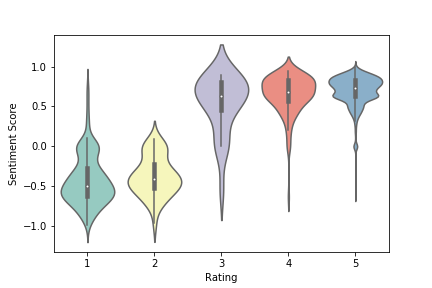
\includegraphics[width=0.7\linewidth]{sentscore_violin.png}
%	\caption{Sentiment Scores and Ratings}
%	\label{fig: sentscore_violinr}
%\end{figure}
% Figure \ref{fig: regplot_text_d_ent_others} displays the relationship between an installer's text-based dispersion and its rating entropy via a scatter plot on a regression line.
%\begin{figure}
%	\centering
%	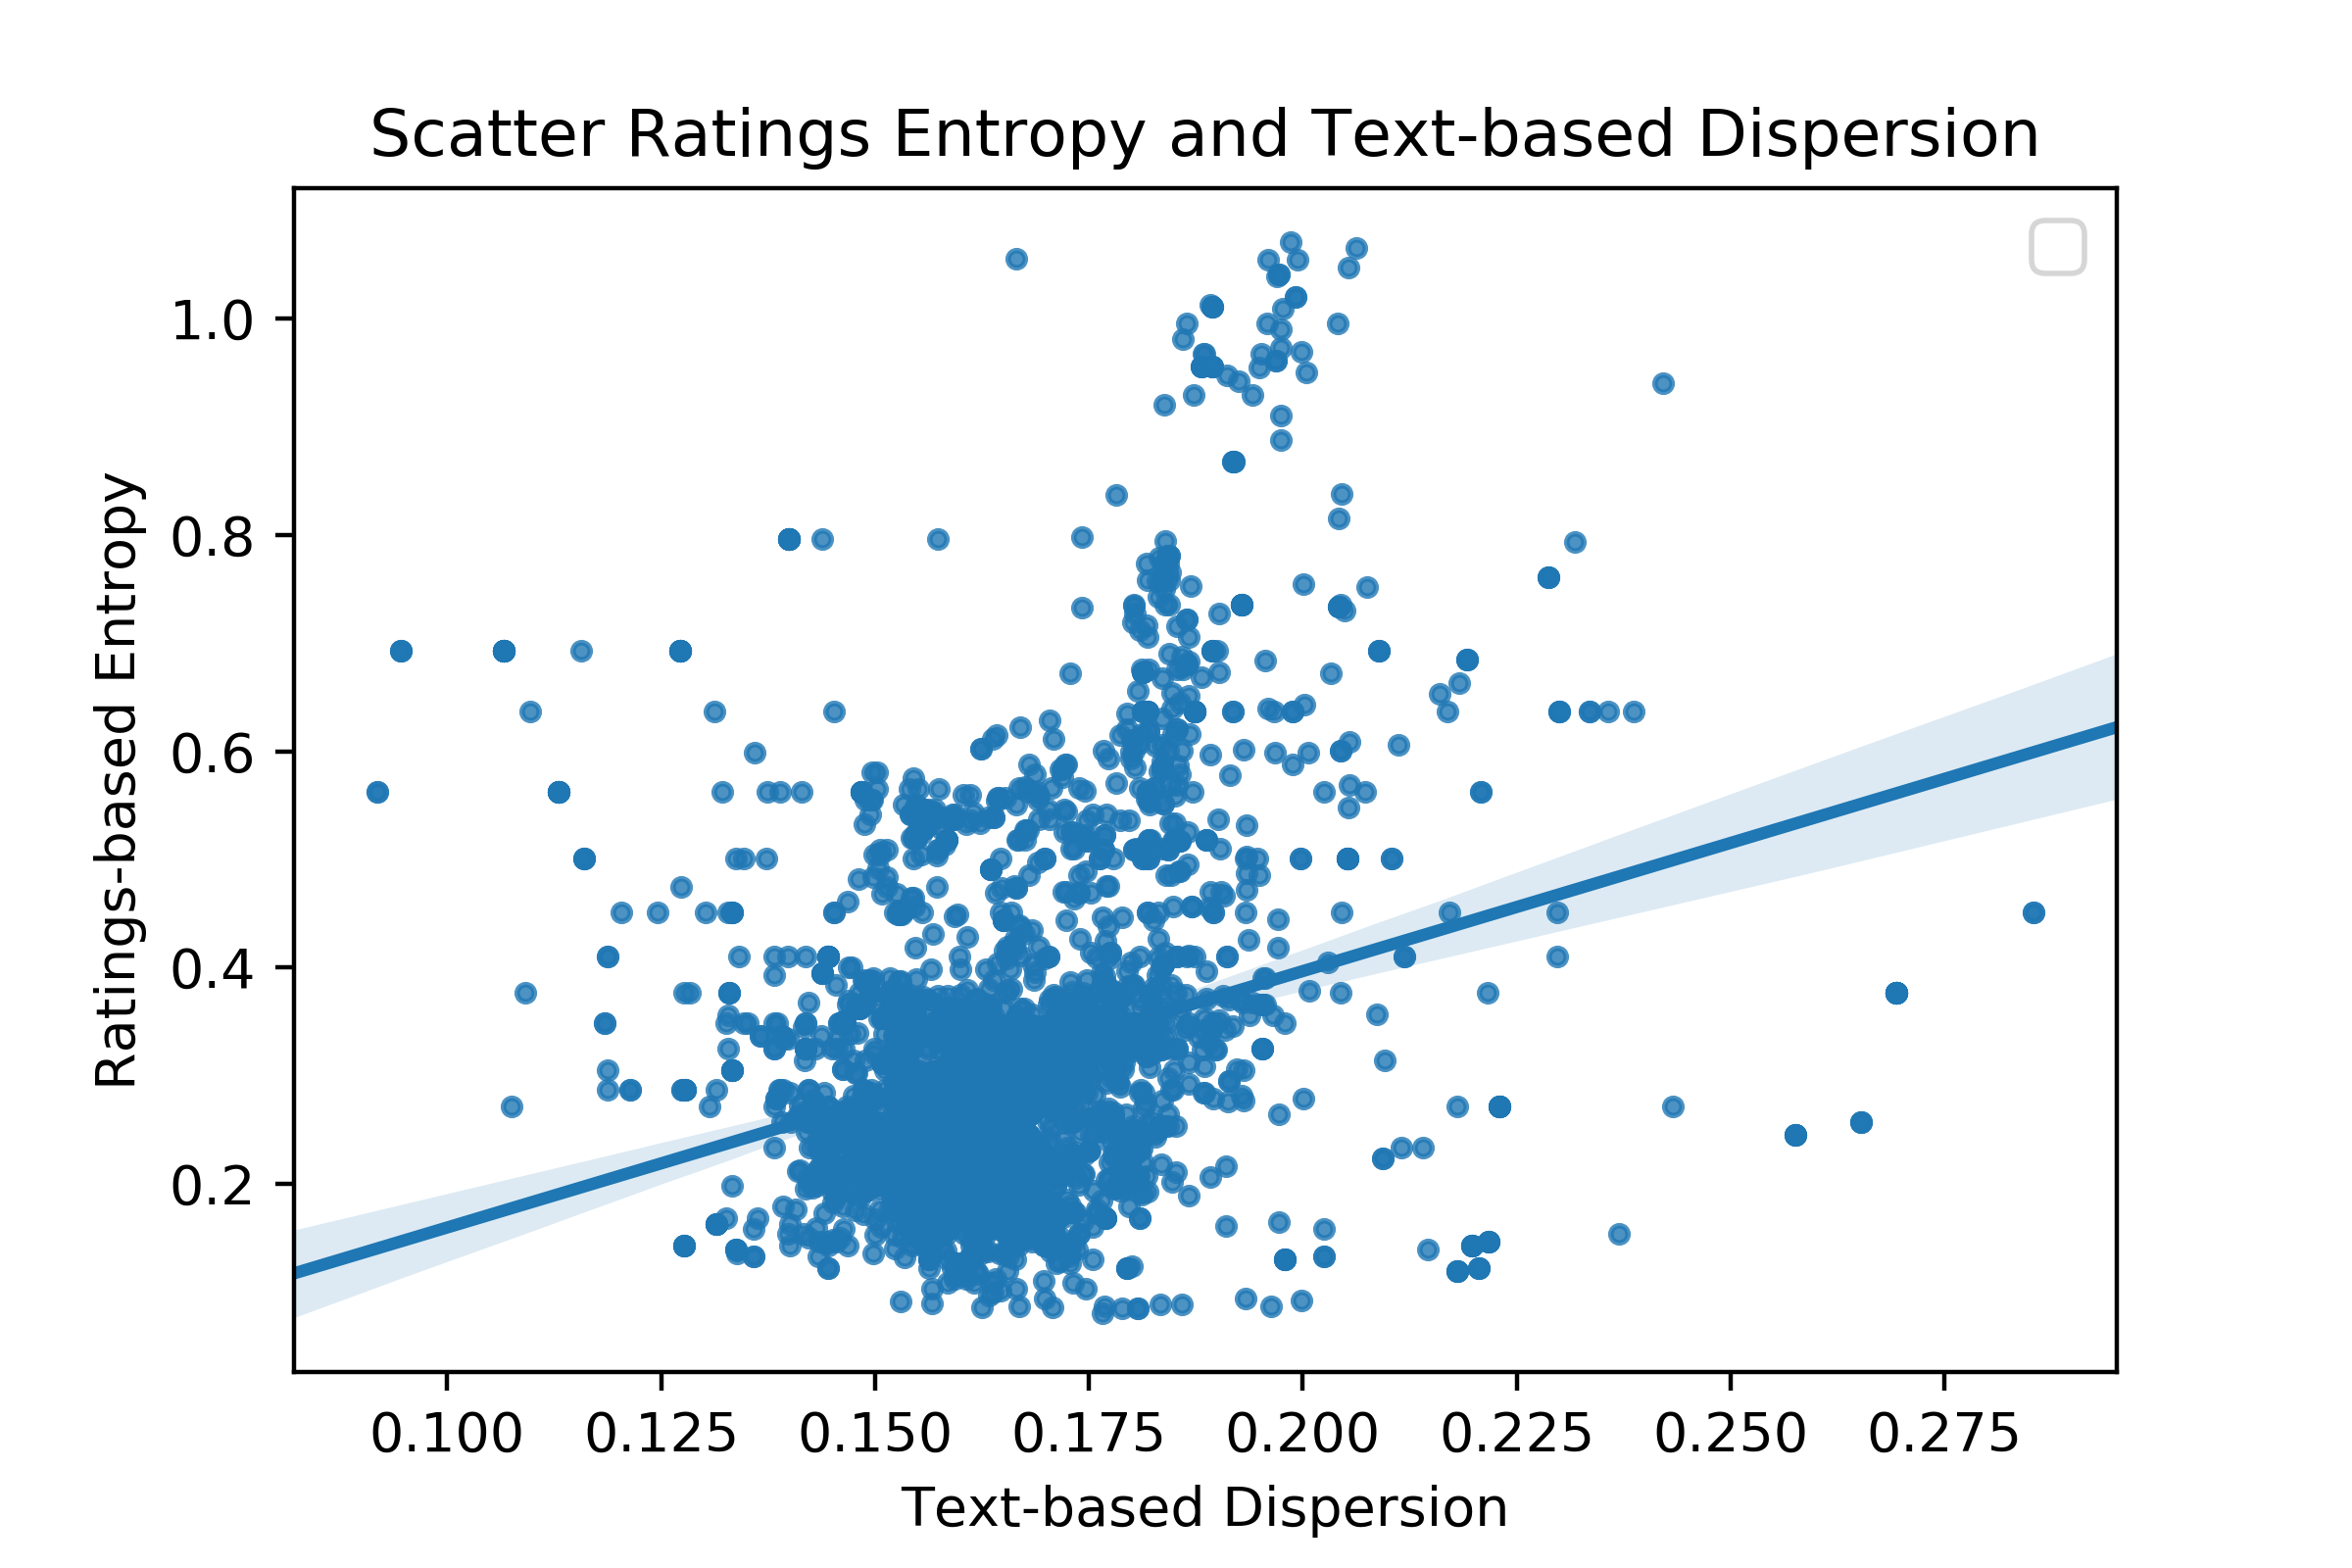
\includegraphics[width=0.7\linewidth]{regplot_text_d_ent_others.png}
%	\caption{Text-based Dispersion and Entropy of Ratings}
%	\label{fig: regplot_text_d_ent_others}
%\end{figure}

\textbf{PLEASE REVIEW THIS PARAGRAPH AND UPDATE IF NECESSARY} Table \ref{reg_ind_withtext} shows the estimation results obtained by using different set of explanatory variables in \eqref{model_ind_textbased}. In each column of Table \ref{reg_ind_withtext}, blank represents the absence of the corresponding explanatory variable in the regression.

Regression estimates in Table \ref{reg_ind_withtext} reveal various findings. First, on average, an installer's rating entropy continues to have an inverted U-shaped impact on the installer's activity level even when the text-based dispersion is also considered. Second, an installer's text-based dispersion has a significant and positive first-order effect on the installer's activity level, whereas it has a significant and negative second-order effect  on the installer's activity level (as $\theta_{5} > 0$ and $\theta_{6} < 0$ are both found to be significant). Combining two, on average, an installer's text-based dispersion also has an inverted-U-shaped impact on its activity level.
Third, as indicated by insignificance of coefficients for ``\text{Average\_Sentiment\_Score\_Self}'' and ``\text{Average\_Sentiment\_Score\_Others}'', installer's average sentiment score or its competitors' average sentiment score does not have a significant impact on the installer's activity level. In fact,  Table \ref{reg_ind_withtext} indicates that an installer's average rating better explains the installer's activity level than its average sentiment score. Thus, text context can be ignored in measuring reviews' average polarity intensity  while it is significant in measuring the review dispersion.

%Fourth, when the text content and numerical ratings are considered together, competitors' rating entropy has an insignificant impact on the installer's activity level.


Table \ref{reg_mkt_textbased} displays the estimates obtained by using different set of explanatory variables in \eqref{reg: market-level-textbased}. There are three key findings. First, the  market-level rating entropy continues to be significant and have an inverted-U-shaped impact on market transactions (and number of matches). Second, on average, although the text-based dispersion has an inverted-U-shaped relationship with market transactions, it has an insignificant impact on market transactions. Thus, the text content does not provide significant value in measuring the review dispersion.  Third, the coefficients for the average market-level rating or average market-level sentiment score are both significant, but the text content better captures the ``signal'' of reviews than numerical ratings in the marketplace.

% installers' activity levels and market transactions can also be attributed to sentiment scores and text-based dispersion measures. We use variables $\text{Avg\_Sent\_Self}_{i,t}$ in place of $\text{Avg\_Rating\_Self}_{i,t}$, $\text{Avg\_Sent\_Others}_{i,m,t}$ in place of $\text{Avg\_Others}_{i,m,t}$ to represent individual ratings in individual level analysis, $\text{Avg\_Sent\_Mkt}_{m,t}$ in place of $\text{Avg\_Mkt}_{m,t}$ in market level analysis, and ran the same regression models. The results are presented in table \ref{reg_ind_withtext} for installer level analysis and table \ref{reg_mkt_textbased} for market level analysis.  \\


 





\section{Robustness Check} \label{Sec: Robustness}

\subsection{Dynamic Panel Model}

The regression model in Section \ref{Sec: Installer-level} considers fixed effect for each installer, and that accounts for time-invariant installer-specific factors that may impact the dependent variable, i.e., installer's activity level. This section extends our regression model  \eqref{model_ind_3} to a dynamic panel model by including lagged dependent variables. The inclusion of these variables aims to consider time-variant unobserved heterogeneity that may influence the dependent variable. In light of this, for the installer-level analysis, the equation we estimate is extended to the following:

\begin{align} \nonumber
&\text{Installer\_Activity}_{i,t+1} \\ \nonumber
 &=\gamma_{0}+\gamma_{1} \text{Installer\_Activity}_{i,t}+ \gamma_{2}\text{Installer\_Activity}_{i,t-1}+
\gamma_{3} \text{Rating\_Entropy\_Self}_{i,t} \\ \nonumber
&+ \gamma_{4} \text{Rating\_Entropy\_Self}_{i,t}^ {2} + \gamma_{5} \text{Rating\_Entropy\_Others}_{i,t}  + \gamma_{6} \text{Rating\_Entropy\_Others}_{i,t}^{2} \\ \label{eq: extended_ind}
&+ \text{Controls}_{i,m,t}+ \epsilon_{i,t+1}.
\end{align}

However,  the inclusion of the lagged dependent variable in the presence of fixed effects may cause endogeneity bias, as such an addition may lead a correlation between the regressors and the error \citep{nickell1981biases}. To overcome this, we use \cite{arellano1991some}'s method for dynamic panel data. \cite{arellano1991some} estimator is a general method of moments estimator that is based on dynamic panel data with first differences. It uses lagged variables as instruments to address the endogeneity bias. A requirement for \cite{arellano1991some} estimation is serially uncorrelation in first-differenced errors. We provide support for this property in Table \ref{autocorrelation_test}.



We also modify the market-level model \eqref{reg: market-level-rating} to include lagged dependent variables:
\begin{align} \nonumber
&\text{Market\_Transaction}_{m,t+1}\\ \nonumber
& =\alpha_{0}+ \alpha_{1} \text{Market\_Transaction}_{m,t}+ \alpha_{2} \text{Market\_Transaction}_{m,t-1} + \alpha_{3} \text{Market\_Transaction}_{m,t-2} \\ \label{eq: ext_market_level}
&+ \alpha_{4} \text{Rating\_Entropy\_Mkt}_{m,t}+ \alpha_{5}\text{Rating\_Entropy\_Mkt}_{m,t} ^2 + \text{Controls}_{m,t}  +\epsilon_{m,t+1}.
\end{align}
To overcome any potential endogeneity bias in this regression, we apply similar steps as the ones explained for the analysis of the installer-level activity. In applying  \cite{arellano1991some} estimator, we included $1-3$ lags of variables.  

Tables \ref{rob_ind_dynamic} and \ref{rob_mkt_dynamic} include our installer-level and market-level estimates. An installer's rating entropy and its competitors' rating entropy continue to have an inverted U-shaped impact on the installer's activity level. Furthermore, there is also an inverted-U-shaped relationship between the market-level rating entropy and market transaction (or number of matches).  Thus, our findings are robust in this extension.



%----

%Staiger D, Stock JH (1997) Instrumental variables regression with weak instruments. Econometrica 65(3):557–586.
%Nickell S (1981) Biases in dynamic models with fixed effects. Econometrica (6):1417–1426.
%Arellano M, Bond S (1991) Some tests of specification for panel data: Monte Carlo evidence and an application to employment equations. The Review of Economic Studies 58(2):277–297
%Bowsher C (2002) On testing overidentifying restrictions in dynamic panel data models. Economics Letters 77(2):211–220
%
%The regression in Eq. 1 includes county fixed effects, ci , to control for unobserved heterogeneity across counties that does not vary across time yet influences the staffing level. The presence of fixed effects in Eq. 1 along with the lagged dependent variables and regressors raises a concern of endogeneity bias in its estimation (Nickell (1981)). We use Arellano and Bond (1991) dynamic panel data model with first differences and lagged variables as instruments to overcome this issue. We limit the number of lags used as instruments in the model (Bowsher (2002)). To be specific, for the voting resource regressors (logVotersPerPW, logAbsentBallotsPerPP, logEarlyBallotsPerPP, logEDBallotsPerPP, logProvBallotsPerPP) we use the second and third lags as instruments (corresponding to both a midterm and presidential election). For voter demographic variables (PctDemocrat, PctWhite), we use the second election lag as an instrument, and for poll worker recruitment difficulty (PollDiff ), we use the most recent election lag as an instrument. We do not include lags of the other regressors (logPersonPerSqMile, HousePrice, MedInc, UseDRE, Pct65Plus) because we believe they should be uncorrelated with shocks to the number of voters or poll workers. The Hansen test (robust to heteroscedasticity) for overidentifying restrictions assumes a null hypothesis that our instruments meet the exogeneity requirement. We do not find evidence that the exogeneity assumption is violated (Table EC.2). We also address two issues with Arellano-Bond estimation. First, it may perform poorly if instruments are weak, which could occur if changes in county election demographics were fully adjustable from one election to the next, thereby having no relation to past values. We believe, however, that county demographics are somewhat rigid over time. Consistent with that view, we do not find evidence of weakness using F-statistics from the first-stage 2SLS regressions of the first differences of each endogenous variable (pooled across counties and election years) on its lagged instrument(s) (see Table EC.3). Second, Arellano-Bond estimation requires serially uncorrelated errors, which is supported (Table EC.2)
%
%To assess the validity of the instruments, we perform
%several statistical tests to examine whether they
%meet the relevance criteria. First, we note that the
%R2 values from the first stage regressions of the four
%endogenous variables lie between 0.55 and 0.70, indicating
%that the instruments have significant explanatory
%power. Second, the F -statistics of the excluded
%instruments in the first stage regressions are well over
%10 in all of our regressions, indicating that the instruments
%are not “weak” in the sense of Staiger and Stock
%(1997). Although not conclusive, these test statistics
%
%
%\url{https://fmwww.bc.edu/GStat/docs/StataIV.pdf}
%\url{https://www.univ-orleans.fr/deg/masters/ESA/CH/Geneve_Chapitre2.pdf}
%\url{https://faculty.fuqua.duke.edu/econometrics/presentations/2013/Rossi-Instruments_and_Fixed_Effects.pdf}
%
%-----




\subsection{Additional Support for Inverted U-Shaped Relationship}

To further validate the inverted U-shaped relationship between an explanatory variable and the response variable, one must check whether the stationary point of the explanatory variable lies within its range in our sample. This check is important to distinguish the inverted U-shaped relationship from a concave monotone relationship.  The ranges of ``\text{Rating\_Entropy\_Self},'' ``\text{Rating\_Entropy\_Others}'' and ``\text{Rating\_Entropy\_Mkt}'' are provided in Tables \ref{sumstats_ind} and \ref{sumstats_mkt}.
Based on our estimates in Sections \ref{Sec: Installer-level} and \ref{Sec: Market-level}, we calculate the stationary points for these variables as \textbf{PLEASE FILL IN BLANKS} $S_{\text{self}} \doteq - \beta_{1}/ (2 \beta_{2}) = 0.272$, $S_{\text{others}} \doteq  - \beta_{3}/(2 \beta_{4}) =0.094 $ and $S_{\text{mkt}} \doteq - \beta_{6}/(2 \beta_{7}) =0.505 $. In fact, stationary point for each of these variables is also evident in Figures \ref{fig: marginsplot_ind_ent_self}, \ref{fig: marginsplot_ind_ent_others} and \ref{fig: marginsplot_mkt_entmkt}. Comparing ranges and the stationary points, we conclude that in our data, the stationary point of each rating entropy variable lies within its observed data range. This provides further validation for the inverted U-shaped relationship we find in Sections \ref{Sec: Installer-level} and \ref{Sec: Market-level}.


We used a common criteria to identify inverted U-shaped relationships.  Some researcher argue that for the inverted U-shaped relationship to be meaningful for an explanatory variable, the stationary point for that variable should not be too close to the end points of the data range or too far from the sample mean (e.g., 3 standard deviation far) \cite{lind2010or}. This concern does not apply our analysis as the stationary point for each rating entropy is close to its sample mean. Specifically, $S_{\text{self}}$, $S_{\text{others}}$ and $S_{\text{mkt}}$ are respectively $1.3$ ,$0.80$ and  $0.73$  standard deviation away from their sample means.






%
%The commonly used criterion for identifying
%an inverted-U-shaped relationship, i.e., the significance
%of the quadratic term that we used in the main analysis,
%has been questioned in some recent literature
%(Lind and Mehlum 2010). This literature argues that
%the quadratic specification may erroneously create an
%extreme point even though the true relationship is
%concave and monotone. We believe that this concern
%does not necessarily apply to our analysis because
%our extreme points are close to the sample means.


%stationary point should lie within the range of the variable
%in our sample.
%To distinguish an increasing concave relationship
%from an inverted U-shaped relationship,
%we compute the stationary points for temporary
%and part-time labor mixes as −1/22 and −3/24
%,
%respectively, for the sales equation and check if
%they lie within the sample. We repeat the process
%for the expense and profitability equations to test
%for U-shaped and inverted U-shaped relationships,
%respectively.
%
%Aiken and West (1991) state that
%to identify a nonmonotonic relationship, the stationary
%point should lie within the meaningful range
%of the variable. To test if the stationary point lies
%in a meaningful range, they suggest computing the
%slope of the curve for different points of the variable
%and ensuring that the slope is significantly different
%from zero and of different signs on either side
%of the stationary point
%
%For example, in the sales
%equation, the slope of the curve is given by 1 +
%22TempMixit, and the standard error is calculated
%as p
%‘11 + 4TempMixit‘12 + 4‘224TempMixit5
%2
%. Here ‘11
%and ‘22 are the variance of 1 and 2
%, respectively, and
%‘12 is the covariance between 1 and 2
%. Table 4(a)
%shows the tests of the simple slopes for temporary
%and part-time labor-mix variables at the stationary
%point, and ±1 SD, minimum, and maximum values
%in the sample. Since the simple slopes on either side
%of the stationary point are statistically significant and
%are of different signs for both temporary and parttime
%labor-mix variables, we can conclude that the
%inverted U-shaped relationship is supported within
%the sample for the sales equation. We repeat the similar
%analysis for the expense equation, and the results
%are reported in Table 4(b). We find that our statistical
%tests confirm the U-shaped relationship for temporary
%labor-mix variable. Since the stationary point




\subsection{Alternative Test for Inverted U-Shaped Relationship: Spline Regression}


Up to this section, we identified an inverted U-shaped relationship between entropy measures and dependent variables by applying a standard technique. That is, by running a polynomial regression, showing the significance of linear and quadratic terms of entropy measure, and identifying the positive sign for the linear term and the negative sign for the quadratic term. See, e.g., \cite{tan2014does} and \cite{kesavan2014volume} that apply this technique. We also perform spline regressions to provide robustness checks on both individual and market level analysis. This robustness check is also standard in the literature \citep{kesavan2014volume}.

Spline regressions use breakpoints (\emph{knots}) to capture the changes in coefficients for different intervals of explanatory variables. We perform spline regressions with 1 knot and with 2 knots. Knots divide data into sub-samples, and the response variable and the explanatory variable of interest are allowed to have a different linear relationship in each sub-sample. For 1 knot, we create two spline variables $\text{Rating\_Entropy\_Others\_S1}$ and  $\text{Rating\_Entropy\_Others\_S2}$, and consider the linear term of either one only in one of the two ranges of the variable. For the installer-level analysis, we plug in either of these spline variables in place of the linear and quadratic terms of $\text{Rating\_Entropy\_Others}$ in \ref{model_ind_3}.  Likewise, we repeat this procedure for $\text{Rating\_Entropy\_Self}$ in the installer-level analysis and  for $\text{Rating\_Entropy\_Mkt}$ in the market-level analysis. We also further extend this alternative testing to consider spline regressions with 2 knots, which require us to create three spline variables for each rating entropy measure.

%By dividing the sample into subsamples through different thresholds or knots and fitting polynomial regression in each subsample.


The results are presented in Tables \ref{rob_spline_ind} and \ref{rob_spline_mkt}. In Table \ref{rob_spline_ind}, we report the spline regression estimates with one knot on $\text{Rating\_Entropy\_Others}$ in column (I) and with one knot on $\text{Rating\_Entropy\_Self}$ in column (II). We find that the coefficient of the first spline is positive and significant while the second one (which is valid above the breakpoint) is negative and significant ($p<0.001)$, supporting the inverted U-shaped relationships between either rating entropy measure and the installer's activity levels. The conclusions are similar when we consider the case with 2 knots as shown in column (III) and (IV) of Table \ref{rob_spline_ind}.  Next, we consider the market-level analysis with results presented in Table \ref{rob_spline_mkt}. For the case with 1 breakpoint for Rating\_Entropy\_Mkt, first positive and then negative and significant ($p<0.001$) coefficients associated with the two splines in column (I) further validate the inverted U-shaped relationship we established on the market-level. We also find that when we move to the case with two breakpoints, the inverted U-shaped relationship is still preserved. \textbf{THIS IS BASED ON OUR CONVERSION TODAY THAT IN THE UPDATED TABLE, THIRD SPLINE WILL BE SIGNIFICANT}


%\subsection{Excluding Inactive Installers}
%
% We now run a robustness check by excluding installers that have been inactive (i.e., made 0 proposals) for the last two months in the online marketplace. With this modification, our regression results are presented in Table \ref{rob_exclude_inactive}.  The results are consistent, especially on the inverted U-shaped relationship between rating entropy self and an installer's activity level.
%
%% The first two columns are results excluding these said installers ( cluster standard errors on market level - column (1); individual level - column (2)) .

\subsection{Alternative Approach to Measure Text-based Dispersion}

In Section \ref{def: entropy}, we measured the text-based dispersion by taking the median of cosine distances. Alternatively, one can consider the mean of cosine distances to measure the text-based dispersion. Table \ref{reg_ind_rob_text_mean} reports the estimation results when the mean (rather than median) of cosine distances is considered in that measurement. Table \ref{reg_ind_rob_text_mean} suggests that our findings in Section \ref{Sec: TextMining} continue to hold. \textbf{PLEASE INCLUDE MARKET-LEVEL TABLE, TOO}



%\subsection{Market Level Alternative Measure of Success}
%
%In the analysis of ratings dispersion on local market level performance, we used total quotes accepted by consumers to measure the success of marketplace. We present results using total quotes given out by installers, and it remains consistent, as table \ref{reg_mkt_alt_measure} shows.






\section{Discussions}

\paragraph{Average Ratings and Sentiment} : Most the specifications concerning the impact of average ratings captured negative (yet statistically insignificant) effects.  Interestingly, the model using sentiment score and Text-based dispersion measures (table \ref{reg_ind_withtext}) have shown more consistent and significant negative coefficients. After we control for other things, being rated higher or viewed more positive is associated with a lower level of activity intensity going forward. \\

\paragraph{Noise in Reviews} The individual level analysis pertain to ratings and reviews dispersion all revealed an inverted-U type of impact.

\paragraph{Noisy Reviews and Marketplace Matching Performance}: from the marketplace's perspective, dispersion in reviews also exhibits an inverted-U type of relationship with market place matches.

\paragraph{Methodology - text mining} To analyze the reviews texts, we incorporated two text mining methods that 1) - gave reviews texts a one-dimensional sentiment score and 2) utilize word embedding model to measure texts similarity with precision. We demonstrated that the text mining tools are great complement to the quantitative data. To our knowledge, it is the first example of using deep learning based text-mining models on business settings in the operations management literature. We demonstrate the versatility of deep learning methods as a complement to traditional text-mining methods.


\bibliographystyle{informs2014} % outcomment this and next line in Case 1
\bibliography{solarlits} % if more than one, comma separated

\newpage

\begin{APPENDIX}{Electronic Companion}
\section{TABLES}
% Please add the following required packages to your document preamble:
% \usepackage{booktabs}
% \usepackage{graphicx}
\begin{table}[H]
\centering
\begin{threeparttable}[t]
\begin{tabular}{@{}lcccc@{}}
\toprule
                            & (I)         & (II)        & (III)       & (IV)        \\
                            & Installer's & Installer's & Installer's & Installer's \\
Variables                   & Activity Level & Activity Level & Activity Level & Activity Level \\ \midrule
Text-based\_Entropy\_Self   & 5.326***    & 5.389***    & 5.014***    & 4.890***    \\
                            & (0.000)     & (0.000)     & (0.000)     & (0.000)     \\
Text-based\_Entropy\_Self$^2$    & -23.71***           & -23.54***              & -20.29***      & -20.40***      \\
                            & (0.000)     & (0.000)     & (0.000)     & (0.000)     \\
Text-based\_Entropy\_Others & -1.288      & -0.989      & -1.640      & -1.955      \\
                            & (0.389)     & (0.509)     & (0.275)     & (0.193)     \\
Text-based\_Entropy\_Others$^2$   & -9.593              & -13.13                 & 1.348          & 5.132          \\
                            & (0.623)     & (0.517)     & (0.944)     & (0.782)     \\
Average\_Rating\_Self       & -0.942***   &             &             & -0.998***   \\
                            & (0.000)     &             &             & (0.000)     \\
Average\_Rating\_Others     & 0.000219    &             &             & -0.00483    \\
                            & (0.991)     &             &             & (0.813)     \\
Average\_Sentiment\_Self    &             & -0.431      & -0.404      &             \\
                            &             & (0.090)     & (0.129)     &             \\
Average\_Sentiment\_Others  &             & 0.111       & 0.0806      &             \\
                            &             & (0.378)     & (0.524)     &             \\
Rating\_Entropy\_Self       &             &             & 2.044***    & 2.161***    \\
                            &             &             & (0.000)     & (0.000)     \\
Rating\_Entropy\_Self$^2$              &                     &                        & -4.246***      & -4.344***      \\
                            &             &             & (0.000)     & (0.000)     \\
Rating\_Entropy\_Others     &             &             & 0.399*      & 0.384*      \\
                            &             &             & (0.033)     & (0.045)     \\
Rating\_Entropy\_Others$^2$          &                     &                        & -2.382***      & -2.376***      \\
                            &             &             & (0.000)     & (0.000)     \\
Review\_Count               & 0.0489***   & 0.0492***   & 0.0420***   & 0.0413***   \\
                            & (0.000)     & (0.000)     & (0.000)     & (0.000)     \\
Experience                  & 0.178***    & 0.175***    & 0.176***    & 0.177***    \\
                            & (0.001)     & (0.001)     & (0.001)     & (0.001)     \\
Price\_Difference           & 0.0952      & 0.101       & 0.125       & 0.118       \\
                            & (0.278)     & (0.247)     & (0.158)     & (0.181)     \\
Market\_LogRevenue          & -0.0164***  & -0.0165***  & -0.0159***  & -0.0158***  \\
                            & (0.000)     & (0.000)     & (0.001)     & (0.001)     \\
Constant                    & 2.374***    & 2.075***    & 2.379***    & 2.649***    \\
                            & (0.000)     & (0.000)     & (0.000)     & (0.000)     \\
Fixed Effect                & Yes        & Yes         & Yes          &Yes \\
State Dummies               & Yes        & Yes        & Yes           &Yes\\                          
Observations                & 4562        & 4562        & 4562        & 4562        \\
Adjusted-R$^2$                          & 0.633       & 0.633       & 0.638       & 0.638       \\
AIC                         & 13202.7     & 13200.9     & 13147.9     & 13147.6     \\
BIC                         & 13292.7     & 13290.8     & 13263.5     & 13263.2     \\ \bottomrule
\end{tabular}%
\begin{tablenotes}
\item Note: $p$-value in parentheses; $^\star p<0.05;^{\star\star} p<0.01;^{\star\star\star} p<0.001$
\end{tablenotes}
\end{threeparttable}
\caption{Installer Level Analysis with Variables Derived from Text Analysis}
\label{reg_ind_withtext}
\end{table} 
% Please add the following required packages to your document preamble:
% \usepackage{booktabs}
% \usepackage{graphicx}
\begin{table}
\centering
\begin{threeparttable}
\begin{tabular}{@{}lccc@{}}
\toprule
                                               & (I)            & (II)           & (III)          \\
                                               & Market    & Market    & Market    \\
Variables                                      & Transaction & Transaction & Transaction \\ \midrule
Rating\_Entropy\_Mkt                         &                       &                       & 1.605***              \\
                                             &                       &                       & (0.000)               \\
Rating\_Entropy\_Mkt$^2$ &                       &                       & -1.622***             \\
                                             &                       &                       & (0.000)               \\
Average\_Rating\_Mkt                         & -0.259                &                       &                       \\
                                             & (0.092)               &                       &                       \\
Average\_Sentiment\_Mkt                      &                       & -1.316**              & -1.180*               \\
                                             &                       & (0.006)               & (0.012)               \\
Average\_Experience                          & 0.0193*               & 0.0148                & 0.00983               \\
                                             & (0.016)               & (0.058)               & (0.196)               \\
Price\_Difference\_Mkt                       & 0.228                 & 0.228                 & 0.292                 \\
                                             & (0.314)               & (0.301)               & (0.182)               \\
Market\_LogRevenue                           & -0.0820               & -0.0652               & -0.0517               \\
                                             & (0.066)               & (0.125)               & (0.214)               \\
Text\_Dispersion\_Mkt                        & 3.014                 & 1.318                 & -1.856                \\
                                             & (0.443)               & (0.736)               & (0.632)               \\
Text\_Dispersion\_Mkt$^2$                    & -7.258                & -3.138                & 3.539                 \\
                                             & (0.420)               & (0.730)               & (0.691)               \\
Constant                                     & 3.124*                & 2.843*                & 2.688*                \\
                                             & (0.024)               & (0.017)               & (0.021)               \\
Fixed Effect                                   & Yes            & Yes            & Yes            \\
State Dummies                                  & Yes            & Yes            & Yes            \\
Observations                                 & 642          & 642          & 642                  \\
Adjusted R$^2$                               & 0.739                 & 0.743                 & 0.750                 \\
AIC                                            & 8853.4         & 8849.3         & 8843.7         \\
BIC                                            & 8925.9         & 8933.9         & 8928.3         \\ \bottomrule
\end{tabular}%
\begin{tablenotes}
\item Note: $p$-value in parentheses; $^\star p<0.05;^{\star\star} p<0.01;^{\star\star\star} p<0.001$
\end{tablenotes}
\end{threeparttable}
\caption{Market Level Analysis with Variables Derived from Text Analysis}
\label{reg_mkt_textbased}
\end{table} 
% Please add the following required packages to your document preamble:
% \usepackage{booktabs}
\begin{table}[]
\centering
\begin{tabular}{@{}lll@{}}
\toprule
Variable                           & VIF  & 1/VIF \\ \midrule
Rating\_Entropy\_Self                & 7.10 & 0.14  \\
Rating\_Entropy\_Self$^2$            & 5.81 & 0.17  \\
Rating\_Entropy\_Others              & 1.83 & 0.55  \\
Rating\_Entropy\_Others$^2$          & 1.46 & 0.68  \\
Average\_Rating\_Self                & 4.59 & 0.22  \\
Average\_Rating\_Others             & 1.40 & 0.71  \\
Reviews\_Count                      & 1.24 & 0.81  \\
Experience                         & 1.46 & 0.68  \\
Price\_Difference                  & 1.03 & 0.97  \\
Market\_LogRevenue                 & 1.65 & 0.61  \\ \bottomrule
\end{tabular}
\caption{VIF table: Installer Level}
\label{vif_ind}
\end{table}
% Please add the following required packages to your document preamble:
% \usepackage{booktabs}
\begin{table}[H]
\centering
\begin{tabular}{@{}lcc@{}}
\toprule
Variable           & VIF  & 1/VIF    \\ \midrule
Rating\_Entropy\_Mkt    & 6.67 & 0.149965 \\
Rating\_Entropy\_Mkt$^2$ & 6.21 & 0.160950 \\
Average\_Rating\_Mkt     & 1.58 & 0.632615 \\
Experience     & 1.46 & 0.685113 \\
Price\_Difference   & 1.01 & 0.986885 \\
Market\_LogRevenue     & 1.45 & 0.690279 \\ \bottomrule
\end{tabular}
\caption{VIF Table:Market level}
\label{vif_mkt}
\end{table} 
% Please add the following required packages to your document preamble:
% \usepackage{booktabs}
\begin{table}[H]
\centering
\begin{tabular}{@{}ccc@{}}
\toprule
\multicolumn{1}{l}{\textbf{Installer Level Dynamic Panel}} & \multicolumn{1}{l}{} & \multicolumn{1}{l}{} \\ \midrule
Order                                   & z                    & $p-value$  \\
$H_{0}$: No correlation between $\Delta_{i,t}$ and $\Delta_{i,t-1}$ & -9.8283  & 0.00 \\
$H_{0}$: No correlation between $\Delta_{i,t}$ and $\Delta_{i,t-2}$  & -0.66053 & 0.5089 \\
 Sargan Test for overidentifying restriction & $\chi^2(1525)$  =  238.2181& 1.000 \\ \midrule
\textbf{Market Level Dynamic Panel}          &    &      \\ \midrule
Order                           & z      & $p-value$  \\
$H_{0}$: No correlation between $\Delta_{i,t}$ and $\Delta_{i,t-1}$  & -2.7882 & 0.01 \\
$H_{0}$: No correlation between $\Delta_{i,t}$ and $\Delta_{i,t-2}$  & 0.04295  & 0.9657 \\
 Sargan Test for overidentifying restriction & $\chi^2(544)$ =  22.77427 & 1.000 \\ \bottomrule
\end{tabular}
\caption{Dynamic Panel Specification Checks
}
\label{autocorrelation_test}
\end{table} 

\newpage

% Please add the following required packages to your document preamble:
% \usepackage{booktabs}
% \usepackage{graphicx}
\begin{table}[H]
\centering
\begin{tabular}{@{}lcccc@{}}
	\toprule
	& (I)            & (II)           & (III)          & (IV)           \\
	& Installer's    & Installer's    & Installer's    & Installer's    \\
	Variables                                & Activity Level & Activity Level & Activity Level & Activity Level \\ \midrule
	Installer\_Activity$_t$                 & 0.510***       & 0.507***       & 0.509***       & 0.502***       \\
	& (0.000)        & (0.000)        & (0.000)        & (0.000)        \\
	Installer\_Activity$_{t-1}$       & 0.0393         & 0.0374         & 0.0363         & 0.0369         \\
	& (0.130)        & (0.155)        & (0.176)        & (0.158)        \\
	Rating\_Entropy\_Self                    &                &                & 1.322**        & 1.351**        \\
	&                &                & (0.006)        & (0.004)        \\
	Rating\_Entropy\_Self$^2$ &                &                & -1.578*        & -1.740*        \\
	&                &                & (0.043)        & (0.026)        \\
	Rating\_Entropy\_Others           &                & 0.733          &                & 0.695          \\
	&                & (0.059)        &                & (0.069)        \\
	Rating\_Entropy\_Others$^2$       &                & -1.300*        &                & -1.253*        \\
	&                & (0.041)        &                & (0.031)        \\
	Average\_Rating\_Self                    & -0.0618***     & -0.0713***     & -0.0662***     & -0.0680***     \\
	& (0.000)        & (0.000)        & (0.000)        & (0.000)        \\
	Average\_Rating\_Others                  & -0.180         & -0.191         & -0.137         & -0.162         \\
	& (0.128)        & (0.138)        & (0.232)        & (0.183)        \\
	Review\_Count                            & 0.0165*        & 0.0175**       & 0.0134*        & 0.0105         \\
	& (0.023)        & (0.007)        & (0.024)        & (0.077)        \\
	Experience                               & -0.0554        & -0.0445        & -0.0564        & -0.0528        \\
	& (0.333)        & (0.424)        & (0.304)        & (0.326)        \\
	Price\_Difference                        & -0.0164        & 0.110          & 0.0736         & 0.0987         \\
	& (0.879)        & (0.324)        & (0.457)        & (0.366)        \\
	Market\_LogRevenue                       & 0.00348        & 0.00349        & 0.00367        & 0.00283        \\
	& (0.606)        & (0.618)        & (0.593)        & (0.681)        \\
	Observations                             & 3757           & 3757           & 3757           & 3757           \\ \bottomrule
\end{tabular}%
\begin{tablenotes}
\item Note: $p$-value in parentheses; $^\star p<0.05;^{\star\star} p<0.01;^{\star\star\star} p<0.001$
\end{tablenotes}
\vspace{10pt}
\caption{Robustness Check - Installer Level Dynamic Panels}
\label{rob_ind_dynamic}
\end{table} 
% Please add the following required packages to your document preamble:
% \usepackage{booktabs}
% \usepackage{graphicx}
\begin{table}[H]
\centering
\begin{threeparttable}[t]
\begin{tabular}{@{}lcc@{}}
\toprule
                         & (I)            & (II)           \\
                         & Market Transaction       & Market Transaction       \\
Variables                &   &   \\ \midrule
Rating\_Entropy\_Mkt     & 1.501***       & 0.751*         \\
                         & (0.000)        & (0.016)        \\
Rating\_Entropy\_Mkt$^2$ & -2.456***      & -1.609***      \\
                         & (0.000)        & (0.000)        \\
Average\_Rating\_Mkt     & -0.207         & -0.141         \\
                         & (0.169)        & (0.476)        \\
Average\_Experience      & 0.0102         & -0.00118       \\
                         & (0.157)        & (0.882)        \\
Price\_Difference\_Mkt   & 0.0349         & -0.313         \\
                         & (0.865)        & (0.089)        \\
Market\_LogRevenue       & -0.0264        & 0.0403         \\
                         & (0.502)        & (0.051)        \\
Market\_Transaction$_{t}$&                & 0.0238         \\
                         &                & (0.685)        \\
Market\_Transaction$_{t-1}$    &                & -0.00533       \\
                         &                & (0.917)        \\
Market\_Transaction$_{t-2}$   &                & 0.198**        \\
                         &                & (0.001)        \\
Market Fixed Effect      & Yes            & No             \\
Weighted State Dummies   & Yes            & Yes            \\
%Constant                 & 2.176**        &                \\
%                         & (0.003)        &                \\
Observations             & 642            & 421            \\ \bottomrule
\end{tabular}%
\begin{tablenotes}
\item Note: $p$-value in parentheses; $^\star p<0.05;^{\star\star} p<0.01;^{\star\star\star} p<0.001$
\end{tablenotes}
\end{threeparttable}
\vspace{10pt}
\caption{Robustness Check - Market Level Dynamic Panels}
\label{rob_mkt_dynamic}
\end{table} 
% Please add the following required packages to your document preamble:
% \usepackage{booktabs}
% \usepackage{graphicx}
\begin{table}[]
\centering
\begin{threeparttable}[t]
\begin{tabular}{@{}lcccc@{}}
\toprule
                           & (I)            & (II)           & (III)          & (IV)           \\ 
                           & Installer's    & Installer's    & Installer's    & Installer's    \\
Variables                  & Activity Level & Activity Level & Activity Level & Activity Level \\ \midrule
Rating\_Entropy\_Others\_1 & 0.512*    &           &          &          \\
                           & (0.013)   &           &          &          \\
Rating\_Entropy\_Others\_2 & -1.934*** &           &          &          \\
                           & (0.000)   &           &          &          \\
Rating\_Entropy\_Self\_1   &           & 1.200***  &          &          \\
                           &           & (0.000)   &          &          \\
Rating\_Entropy\_Self\_2   &           & -3.072*** &          &          \\
                           &           & (0.000)   &          &          \\
Rating\_Entropy\_Others\_1 &           &           & 0.834*** &          \\
                           &           &           & (0.001)  &          \\
Rating\_Entropy\_Others\_2 &           &           & -1.164*  &          \\
                           &           &           & (0.017)  &          \\
Rating\_Entropy\_Others\_3 &           &           & -1.763*  &          \\
                           &           &           & (0.020)  &          \\
Rating\_Entropy\_Self\_1   &           &           &          & 1.746*** \\
                           &           &           &          & (0.000)  \\
Rating\_Entropy\_Self\_2   &           &           &          & -1.015   \\
                           &           &           &          & (0.099)  \\
Rating\_Entropy\_Self\_3   &           &           &          & -4.641** \\
                           &           &           &          & (0.008)  \\
Observations               & 4562      & 4562      & 4562     & 4562     \\
Adjusted R$^2$                         & 0.631     & 0.633     & 0.632    & 0.633    \\
AIC                       & 13222.5   & 13204.4   & 13218.4  & 13203.5  \\
BIC                        & 13306.0   & 13287.9   & 13308.3  & 13293.4 \\ \bottomrule
\end{tabular}%
\begin{tablenotes}
\item Note: $p$-value in parentheses; $^\star p<0.05;^{\star\star} p<0.01;^{\star\star\star} p<0.001 $
\end{tablenotes}
\end{threeparttable}
\caption{Alternative Inverted-U Testing: Spline Regressions (Installer Level)}
\label{rob_spline_ind}
\end{table}
% Please add the following required packages to your document preamble:
% \usepackage{booktabs}
% \usepackage{graphicx}
\begin{table}[]
\centering
 \begin{threeparttable}[t]
\begin{tabular}{@{}lcc@{}}
\toprule
                        & (I)            & (II)           \\ 
                        & Market Transaction       & Market Transaction       \\
Variables               &   &   \\ \midrule
Rating\_Entropy\_Mkt\_1 & 1.197***       &                \\
                        & (0.000)        &                \\
Rating\_Entropy\_Mkt\_2 & -1.144**       &                \\
                        & (0.008)        &                \\
Rating\_Entropy\_Mkt\_1 &                & 2.157***       \\
                        &                & (0.000)        \\
Rating\_Entropy\_Mkt\_2 &                & -2.100***      \\
                        &                & (0.000)        \\
Rating\_Entropy\_Mkt\_3 &                & 0.356          \\
                        &                & (0.606)        \\
Observations            & 642            & 642            \\
Adjusted R$^2$             & 0.720          & 0.732          \\
AIC                     & 1101.0         & 1074.3         \\
BIC                     & 1136.7         & 1114.4         \\ \bottomrule
\end{tabular}%
\begin{tablenotes}
\item Note: $p$-value in parentheses; $^\star p<0.05;^{\star\star} p<0.01;^{\star\star\star} p<0.001 $
\end{tablenotes}
\end{threeparttable}
\caption{Alternative Inverted-U Testing: Spline Regressions (Market Level)}
\label{rob_spline_mkt}
\end{table}
% Please add the following required packages to your document preamble:
% \usepackage{booktabs}
\begin{table}[]
\centering
\begin{threeparttable}[t]
\begin{tabular}{@{}lccc@{}}
\toprule
 & (I) & (II) & (III) \\ 
 & Market   & Market    & Market    \\ 
 Variables &Transaction & Transaction & Transaction \\ \midrule
Rating\_Entropy\_Mkt  & 4.189** & 4.290** &  \\
 & (0.003) & (0.004) &  \\
Rating\_Entropy\_Mkt$^2$ & -4.066* & -4.147* &  \\
 & (0.020) & (0.018) &  \\
Text\_Dispersion\_Mkt &  &  & 20.57 \\
 &  &  & (0.348) \\
Text\_Dispersion\_Mkt$^2$ &  &  & -61.58 \\
 &  &  & (0.332) \\
Average\_Rating\_Mkt & -0.218 &  &  \\
 & (0.695) &  &  \\
Average\_Sentiment\_Mkt &  & -0.217 & 0.349 \\
 &  & (0.651) & (0.601) \\
Experience & 0.0559* & 0.0573* & 0.0740** \\
 & (0.017) & (0.013) & (0.002) \\
Price\_Difference & 0.0970 & -0.00130 & -0.000982 \\
 & (0.832) & (0.998) & (0.998) \\
 Market\_LogRevenue & -0.282** & -0.288** & -0.379** \\
 & (0.008) & (0.004) & (0.005) \\
Constant & 6.594* & 5.596*** & 3.642 \\
 & (0.019) & (0.000) & (0.053) \\
State Dummies  & Yes        & Yes        & Yes        \\
Fixed Effects  & Yes        & Yes        & Yes        \\
Observations & 746 & 767 & 961 \\ \bottomrule
\end{tabular}
\begin{tablenotes}
\item Note: $p$-value in parentheses; $^\star p<0.05;^{\star\star} p<0.01;^{\star\star\star} p<0.001 $
\item The observation number are higher because the records of winning quotes, by design, is only a small fraction of transaction quotes.  
\end{tablenotes}
\caption{Market Level Use Given Quotes( instead of winning quotes) }
\end{threeparttable}
\label{reg_mkt_alt_measure}
\end{table}
% Please add the following required packages to your document preamble:
% \usepackage{booktabs}
\begin{table}[]
\centering
\begin{threeparttable}
\begin{tabular}{@{}lccc@{}}
\toprule
                  & (I)      & (II)    & (III)   \\
& Installer's Activity & Installer's Activity & Installer's Activity \\
Variables & Level    & Level   & Level   \\ \midrule
Text\_Dispersion\_Self                                 &            & 11.42*     & 13.28*     \\
                                                           &            & (0.032)    & (0.016)    \\
Text\_Dispersion\_Self$^2$    &            & -34.86*    & -37.87*    \\
                                                           &            & (0.019)    & (0.013)    \\
Text\_Dispersion\_Other                                & 14.22      & 13.10      & 14.26      \\
                                                           & (0.086)    & (0.113)    & (0.080)    \\
Text\_Dispersion\_Other$^2$  & -59.45*    & -54.83     & -57.21*    \\
                                                           & (0.035)    & (0.051)    & (0.039)    \\
Average\_Rating\_Self                                             & -0.436     & -0.489     &            \\
                                                           & (0.086)    & (0.062)    &            \\
Average\_Rating\_Others                                    & -0.0164    & -0.0166    &            \\
                                                           & (0.468)    & (0.466)    &            \\
Average\_Sentiment\_Self                                   &            &            & 0.268      \\
                                                           &            &            & (0.438)    \\
Average\_Sentiment\_Others                                 &            &            & 0.0770     \\
                                                           &            &            & (0.802)    \\
Reviews\_Count                                              & 0.0472*    & 0.0450*    & 0.0466*    \\
                                                           & (0.000)    & (0.000)    & (0.000)    \\
Experience                                                 & 0.104      & 0.0946     & 0.100      \\
                                                           & (0.124)    & (0.164)    & (0.144)    \\
Price\_Differences                                         & -0.00831   & 0.0141     & 0.0249     \\
                                                           & (0.936)    & (0.893)    & (0.814)    \\
Market\_LogRevenue                                         & -0.0162*   & -0.0158*   & -0.0156*   \\
                                                           & (0.002)    & (0.002)    & (0.002)    \\
Constant                                                   & 1.507*     & 0.747      & 0.236      \\
                                                           & (0.029)    & (0.348)    & (0.782)    \\
State Dummies  & Yes        & Yes        & Yes        \\
Fixed Effects  & Yes        & Yes        & Yes        \\
Adjusted R$^2$                                             & 0.668      & 0.669      & 0.670      \\
AIC                                                        & 8853.4     & 8849.3     & 8843.7     \\
BIC                                                        & 8925.9     & 8933.9     & 8928.3     \\ \bottomrule
\end{tabular}
\begin{tablenotes}
\item Note: $p$-value in parentheses; $^\star p<0.05;^{\star\star} p<0.01;^{\star\star\star} p<0.001 $
\item The text-based dispersion variables are derived by taking the mean, instead of median, of the pairwise cosine distances.
\end{tablenotes}
\end{threeparttable}
\vspace{10pt}
\caption{Robustness Check - Installer Level Analysis with Text-based Dispersion from Mean Cosine Distances}
\label{reg_ind_rob_text_mean}
\end{table} 
% Please add the following required packages to your document preamble:
% \usepackage{booktabs}
% \usepackage{graphicx}
\begin{table}[]
\centering
\begin{threeparttable}[t]
\begin{tabular}{@{}lccc@{}}
\toprule
                                                     & (I)            & (II)           & (III)          \\ 
                                                     & Installer's    & Installer's    & Installer's    \\
Variables                                            & Activity Level & Activity Level & Activity Level \\ \midrule
Rating\_Entropy\_Self                                &                &                & 1.428***       \\
                                                     &                &                & (0.000)        \\
Rating\_Entropy\_Self$^2$                            &                &                & -2.590***      \\
                                                     &                &                & (0.000)        \\
Rating\_Entropy\_Others                              &                & 0.386          & 0.358          \\
                                                     &                & (0.085)        & (0.108)        \\
Rating\_Entropy\_Others$^2$                          &                & -2.243***      & -2.312***      \\
                                                     &                & (0.000)        & (0.000)        \\
Average\_Rating\_Self                                & -0.551**       & -0.524*        & -0.489*        \\
                                                     & (0.007)        & (0.011)        & (0.033)        \\
Average\_Rating\_Others                              & 0.00733        & 0.000713       & 0.0000629      \\
                                                     & (0.741)        & (0.977)        & (0.998)        \\
Review\_Count                                        & 0.0504***      & 0.0479***      & 0.0436***      \\
                                                     & (0.000)        & (0.000)        & (0.000)        \\
Experience                                           & 0.136*         & 0.134*         & 0.133*         \\
                                                     & (0.010)        & (0.012)        & (0.012)        \\
Price\_Difference                                    & 0.188*         & 0.200*         & 0.208*         \\
                                                     & (0.036)        & (0.027)        & (0.021)        \\
Market\_LogRevenue                                   & -0.00645       & -0.00618       & -0.00553       \\
                                                     & (0.148)        & (0.165)        & (0.216)        \\
Constant                                             & 2.788***       & 2.868***       & 2.995***       \\
                                                     & (0.000)        & (0.000)        & (0.000)        \\
Fixed Effect                                         & Yes            & Yes            & Yes            \\
State Dummies                                        & Yes            & Yes            & Yes            \\
Observations                                         & 3472           & 3472           & 3472           \\
Adjusted R$^2$                                          & 0.622          & 0.625          & 0.627          \\
AIC                                                  & 9693.2         & 9670.1         & 9655.4         \\
BIC                                                  & 9748.6         & 9737.7         & 9735.3         \\ \bottomrule
\end{tabular}%
\begin{tablenotes}
\item Note: $p$-value in parentheses; $^\star p<0.05;^{\star\star} p<0.01;^{\star\star\star} p<0.001 $
\end{tablenotes}
\caption{Robustness Check Excluding Inactive Installers}
\end{threeparttable}
\label{rob_exclude_inactive}
\end{table}


%\section{Tests for Fixed and Random Effects in \eqref{model_ind_3}}\ref{Apx: Hausman}
%
% Individual Level - FE vs RE Hausman Test\\
% $H_o$:  difference in coefficients not systematic
%\begin{align*}
%\chi^{2}(13) = (b-B)'[(V_b-V_B)^(-1)](b-B)=44.23\\
%Prob>\chi^{2} =0.0000
%\end{align*}
%Market Level -FE vs. RE Hausman Test\\
% $H_o$:  difference in coefficients not systematic
%\begin{align*}
%\chi^{2}(18) = (b-B)'[(V_b-V_B)^(-1)](b-B)=      403.30\\
%Prob>\chi^{2} =0.0000
%\end{align*}
%
%\label{Apx: Hausman}
%\textbf{PLEASE INSERT A TABLE THAT REPORTS THE TEST RESULTS}


%
%\section{My Earlier Question}
%
%What is the total number of proposals in each year?
%Which state is number \#1 in terms of total wins/total proposals?
%Which state is worst in terms of total wins/total proposals?
%Q1) IF THEY OPERATE AT MULTIPLE LOCATIONS, DO THEY PROVIDE
%THAT INFO ON THEIR PROFILE? \\
%We do not have info if they operated on multiple locations or not. I scrape their headquarter address , with ZIP code info.
%Q2) WHAT IS THE FORMAT OF THE LOCATION INFO - IS IT A DETAILED
%ONE WITH A ZIPCODE? PLEASE INCLUDE AN EXAMPLE FOR ME HERE. \\
%Emerald Energy of North Carolina Headquarters
%2624 Leighton Ridge Drive, Suite 120
%Wake Forest, NC
%27587 US
%
%COULD YOU PLEASE PREPARE THESE TWO GRAPHS? 1) TOTAL NUMBER
%OF REVIEWS PER INSTALLER - MAX NUMBER OF REVIEW FOR AN IN-
%STALLER AND HISTOGRAM? 2) NUMBER OF INSTALLERS IN EACH STATE
%FOR TOP 10 STATES \\
%QUESTIONS: 1) HOW MANY OF THE INSTALLERS DO NOT HAVE A RE-
%VIEW? 2) WHAT IS THE PERCENTAGE OF THOSE INSTALLERS IN THE LO-
%CAL MARKET WIN AND SUBMITTED PROPOSALS? 3) WHAT DO YOU AS-
%SUME ABOUT THEM IN THE EMPIRICAL ANALYSIS? \\
%We didn't need to assume anything. I just computed all the variables the way as we stated. \\
%All installers started with 0 reviews, naturally. \\
%If we look at the observations that are included in the analysis, less than 5 percent of observations have 0 reviews ( mostly due to its newly established). \\
%If we look at the end of the panel, only 1 installer has 0 reviews, and have a positive entothers value ( hence is included in the analysis)
%\textbf{YOU MENTIONED controls are to capture factors that are irrelevant to the rating entropy. Is Experience really irrelevant to the rating entropy?? }

\end{APPENDIX}


\clearpage
% Appendix here
% Options are (1) APPENDIX (with or without general title) or
%             (2) APPENDICES (if it has more than one unrelated sections)
% Outcomment the appropriate case if necessary
%
% \begin{APPENDIX}{<Title of the Appendix>}
% \end{APPENDIX}
%
%   or
%
% \begin{APPENDICES}
% \section{<Title of Section A>}
% \section{<Title of Section B>}
% etc
% \end{APPENDICES}


% Acknowledgments here
\ACKNOWLEDGMENT{ .}


% References here (outcomment the appropriate case)

% CASE 1: BiBTeX used to constantly update the references
%   (while the paper is being written).
%\bibliographystyle{informs2014} % outcomment this and next line in Case 1
%\bibliography{<your bib file(s)>} % if more than one, comma separated

% CASE 2: BiBTeX used to generate mypaper.bbl (to be further fine tuned)
%\input{mypaper.bbl} % outcomment this line in Case 2

%If you don't use BiBTex, you can manually itemize references as shown below.





%%%%%%%%%%%%%%%%%
\end{document}
%%%%%%%%%%%%%%%%%

